\chapter{User Documentation}
In the first part, the chapter provides a description of the two showcase games with the way they are controlled. The second part will then lead the user of the framework step by step through creating a scene. It serves as an introduction to the way TaleCraft works. Finally, the third part then introduces the framework itself in detail with all its features.


\section{Showcase}
To demonstrate the capabilities of our framework, we chose to recreate scenes from two classic point-and-click adventure games: \textit{The Secret of Monkey Island} and \textit{Beneath a Steel Sky}. Both titles are iconic representatives of the genre, released during its golden era, and introduced several innovative features that later became genre standards. While \textit{The Secret of Monkey Island} uses a command-based interaction system, \textit{Beneath a Steel Sky} takes a more context-sensitive approach. The two games also differ in their inventory design and other small UI elements, such as interaction tags and descriptive sentences, making them ideal candidates to test and showcase the flexibility of our framework.

Another reason we selected these specific titles is their age and current distribution status: they are no longer sold as new releases. Works in the public domain can be used freely without restrictions, but since video games are still a relatively young medium, only a few very old titles or special cases have entered the public domain.
Our framework is non-commercial and our use of these games falls under fair use for educational purposes, but the boundaries of fair use are not always clearly defined. 
Newer game developers might object to similar use of their intellectual property. We encourage all readers to support the original games where possible. The sequel to \textit{Beneath a Steel Sky} named \textit{Beyond a Steel Sky} is available on Steam \cite{Beyond-a-Steel-Sky}, and \textit{The Secret of Monkey Island} can be purchased on Steam as a modern remake \cite{TSoMI-steam}.

\subsection{Instructions}
The \verb|Build| folder inside \verb|Attachments.zip| includes the \verb|Build-TSoMI| and \verb|Build-BaSS| directories, which in addition to other files contain an executable file. To run the game, simply click on the \verb|TaleCraft.exe| binary in ether of the folders. Both games will display a \textit{Made with Unity }splash screen followed by the scene itself. To quit the game, the player needs to simply press the Esc key on the keyboard.

\subsection{Beneath a Steel Sky}
\textbf{Beneath a Steel Sky} showcase takes place in a starting location of the original game. The style of the following instructions is adapted from the original manual for the game \cite{BaSS-Manual}.

\textbf{Clicking} on objects or characters causes the main character, Foster, to interact with them. To \textbf{move} Foster, the player can point the cursor at navigable areas of the screen and click either mouse button. Foster will not walk into walls or inaccessible areas. Certain objects in the game world can be \textbf{examined} or \textbf{interacted} with. These are identified by on-screen tags that appear when the cursor hovers over them. Pressing the \textbf{left mouse button} causes Foster to examine the object, while the \textbf{right mouse button} attempts to pick up or use it. The game selects the most logical action based on context, for example, clicking on a character will typically initiate a conversation. 

When the pointer is moved to the top edge of the screen, a horizontal bar appears, which represents an \textbf{inventory} (see Figure \ref{fig:BaSS-manual}). It contains items currently carried by Foster and interaction with them follows the same logic as with objects in the game world: \textbf{hovering} the cursor over an item reveals its name, pressing the \textbf{left mouse button} displays a short description of the item, while pressing the \textbf{right mouse} button selects it for further interaction. 

When the cursor hovers over another character, clicking either mouse button initiates a conversation. Dialogue options are presented at the top of the screen and the player can choose a line by clicking on it. 

\begin{figure}[H]
\centering
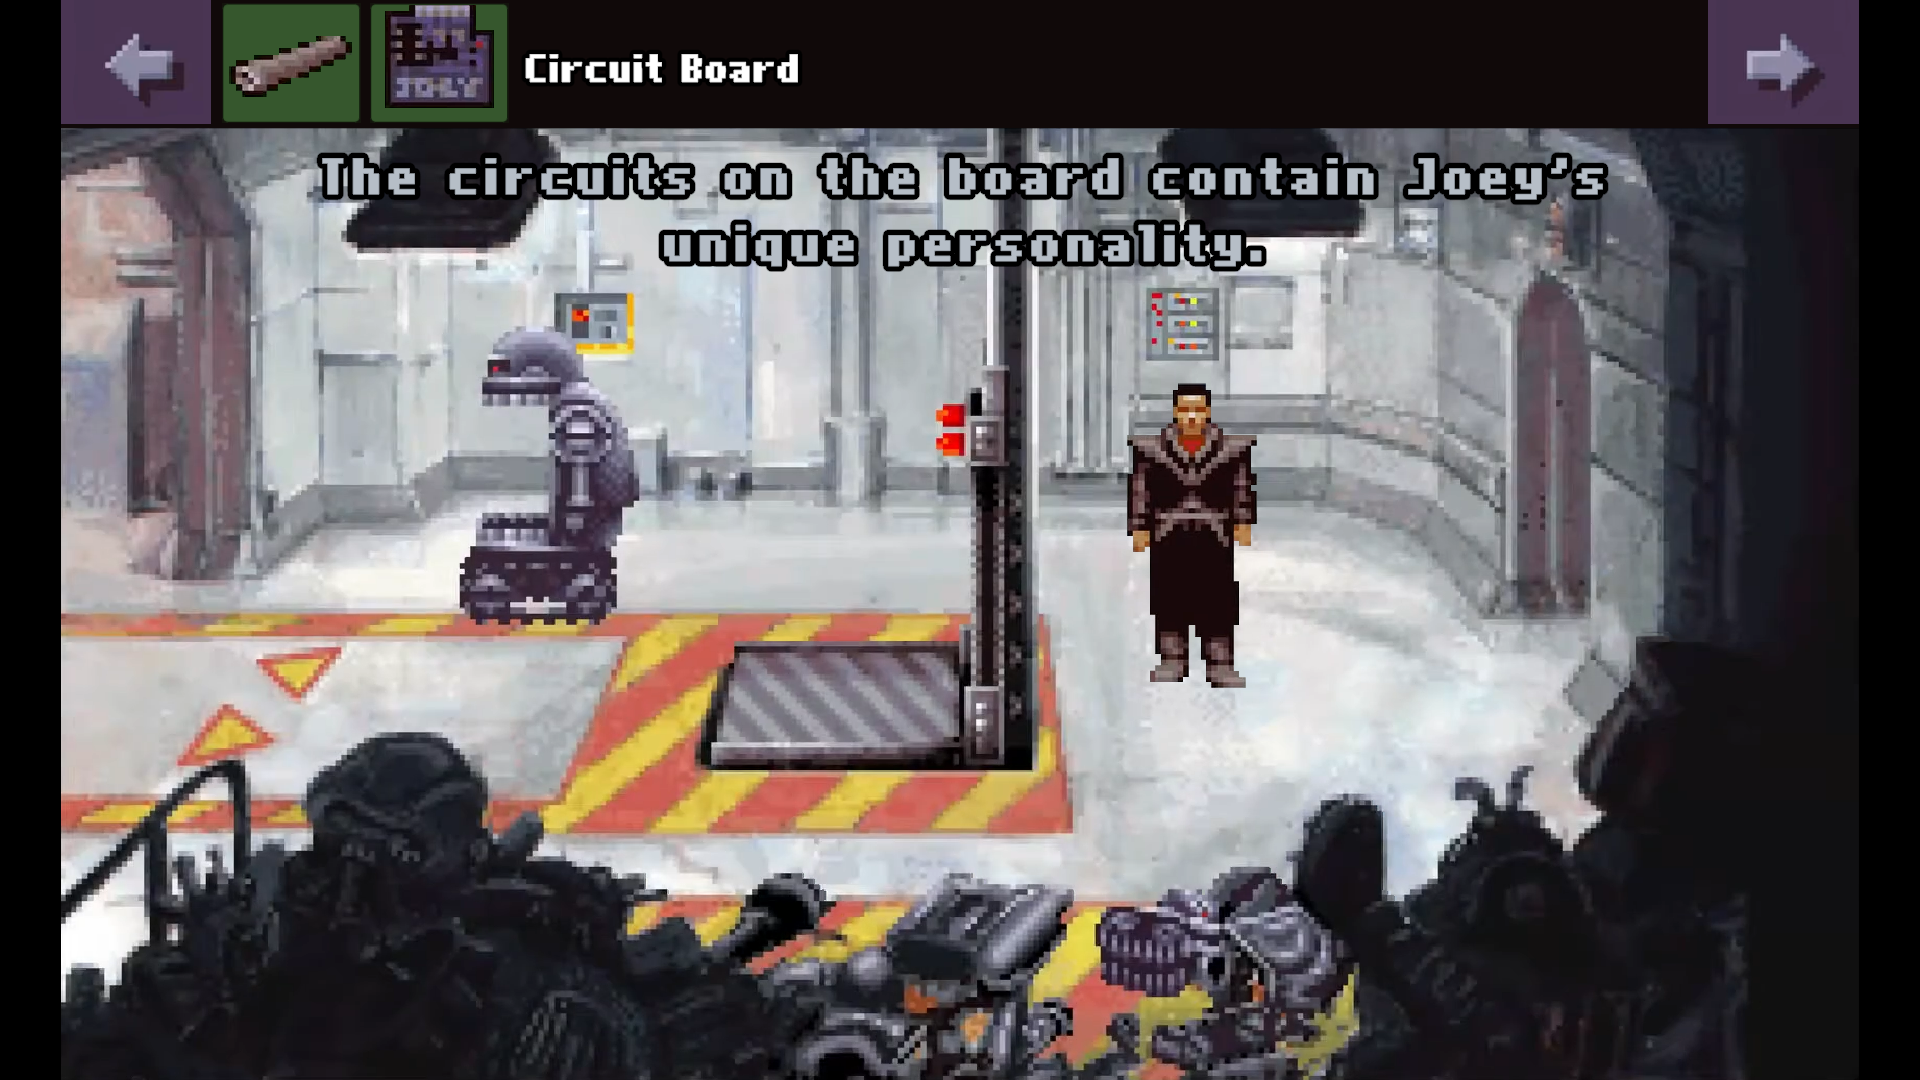
\includegraphics[width=.8\linewidth]{img/manual.png}
\caption{Beneath a Steel Sky (showcase): Screen.}
\label{fig:BaSS-manual}
\end{figure}

\subsection{The Secret of Monkey Island}
The showcase game of The Secret of Monkey Island takes place on a street in the Town of Maleé. The style of the following instructions is adapted from the original manual for the game \cite{TSoMI-Manual}.

\subsubsection{Screen}
The game screen is divided into multiple visually distinct parts (see Figure \ref{fig:TSoM-manual}):
\begin{enumerate}
    \item \textbf{Animation window} is the largest area of the screen and serves as the main stage where the action occurs. It displays the current location the protagonist, Guybrush, is currently in. All character dialogue and game-related messages are also displayed in this window. 
    \item Located directly below the Animation window, the \textbf{Sentence} is where players construct simple commands that guide Guybrush's actions. A typical sentence includes a verb and one or two objects. For example, a valid command might be: “\verb|Look at poster.|”
    \item \textbf{Command verbs} are listed in columns underneath the Sentence. Players select verbs by hovering the cursor over them and clicking the left mouse button.
    \item The \textbf{Inventory} is located to the right of the Command verbs section. There is no limit to how many items can carried. When more than six items are in the inventory, arrow buttons appear to allow scrolling through the full list. 
\end{enumerate}

\begin{figure}[H]
\centering
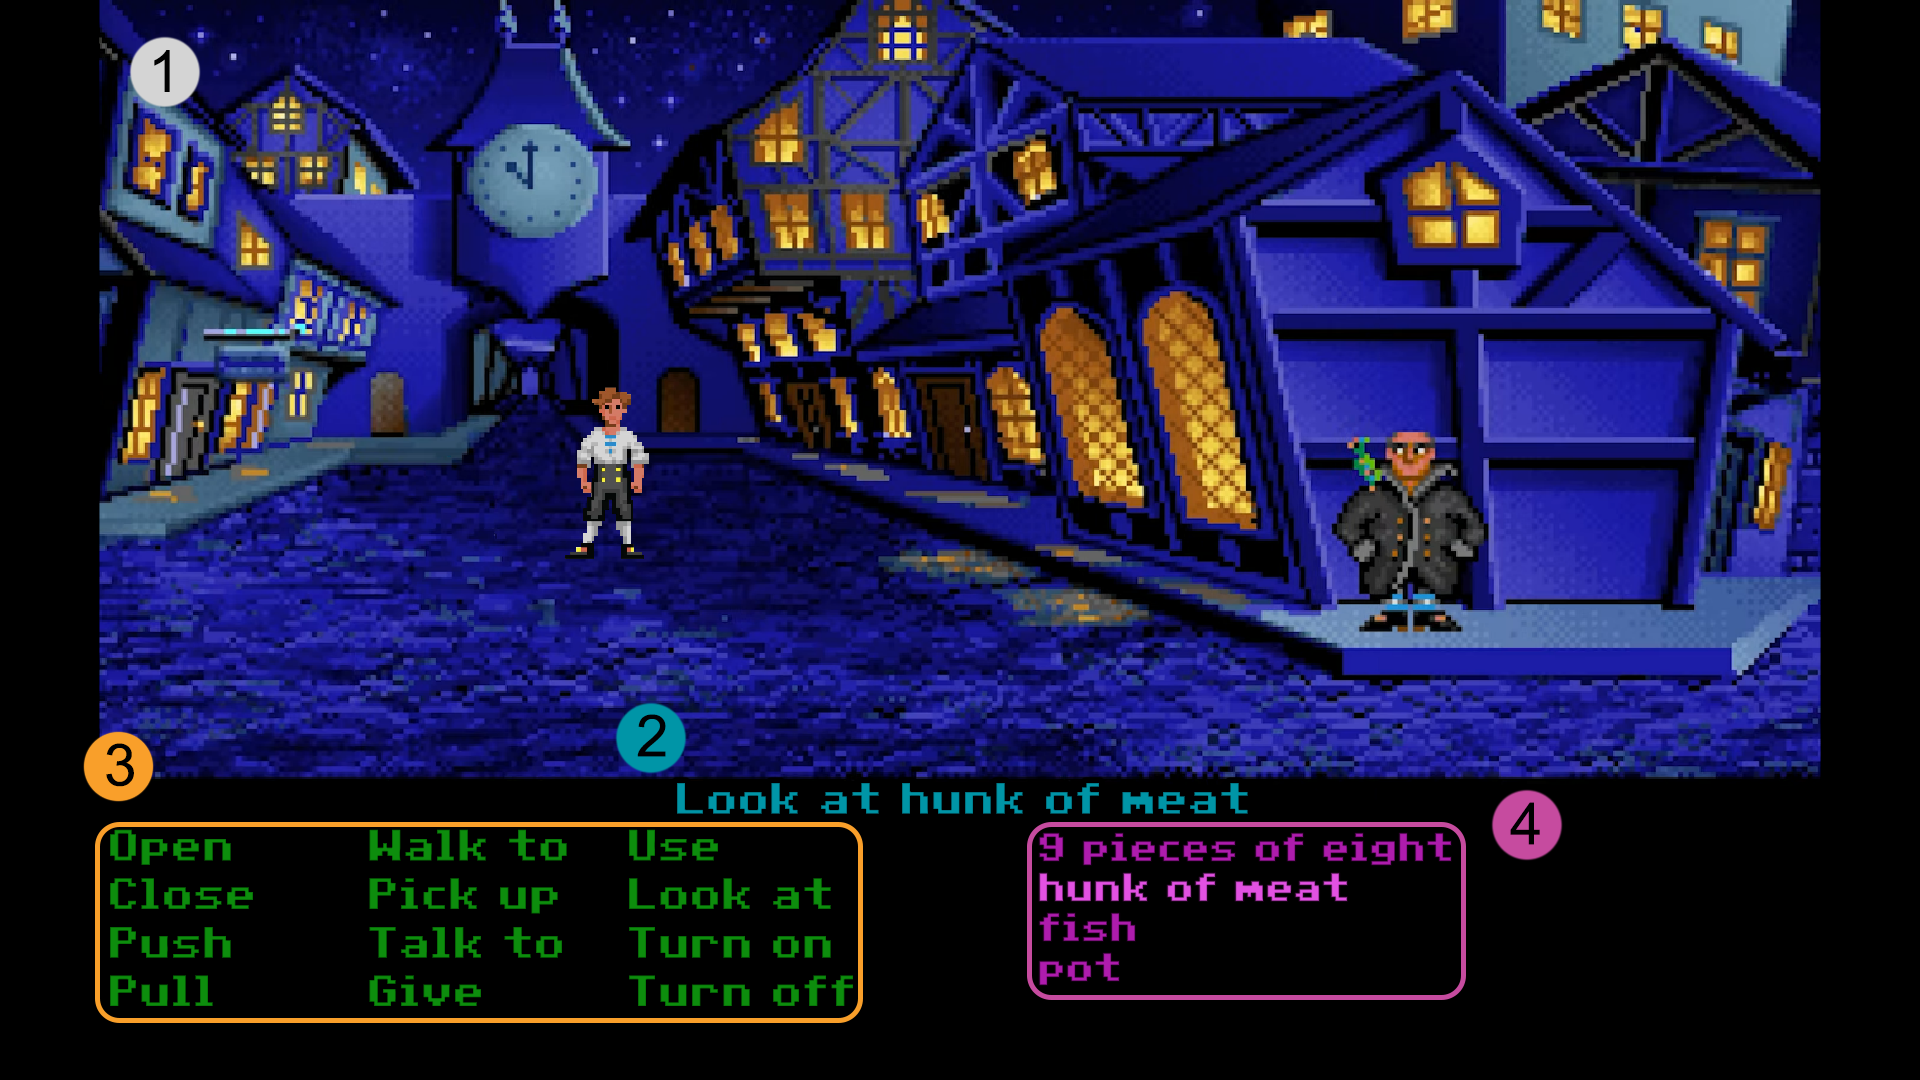
\includegraphics[width=.8\linewidth]{img/tutorial-tsomi.png}
\caption{The Secret of Monkey Island (showcase): Screen.}
\label{fig:TSoM-manual}
\end{figure}

\textbf{Noun Selection and Character Interaction}
Objects, also referred to as nouns, can be selected in two ways. The most common method is by moving the cursor over an object in the Animation window. Most interactive objects in the environment have names, and if an object is usable, its name will appear in the \textit{Sentence} when the player hovers over it. If no name appears, the object is likely part of the background and serves no gameplay purpose. The objects from the Inventory can be selected directly by clicking on them.

\subsubsection{Movement}
To move Guybrush around the world, the cursor needs to be pointed to the desired location followed by a click. \textit{Walk to} is the default verb in the Command sentence, as moving is the most frequent action players will perform.

\subsubsection{Talking to Characters}
To talk to another character, the player can select Talk to command, move the pointer over them and press the left mouse button. During a conversation, dialogue options will appear at the bottom of the screen as seen in Figure \ref{fig:TSoM-manual2}.  The phrase that we want Guybrush to say can be selected by simply clicking on it. What Guybrush says can influence how other characters respond, and new dialogue options may appear as conversations develop.

\begin{figure}[H]
\centering
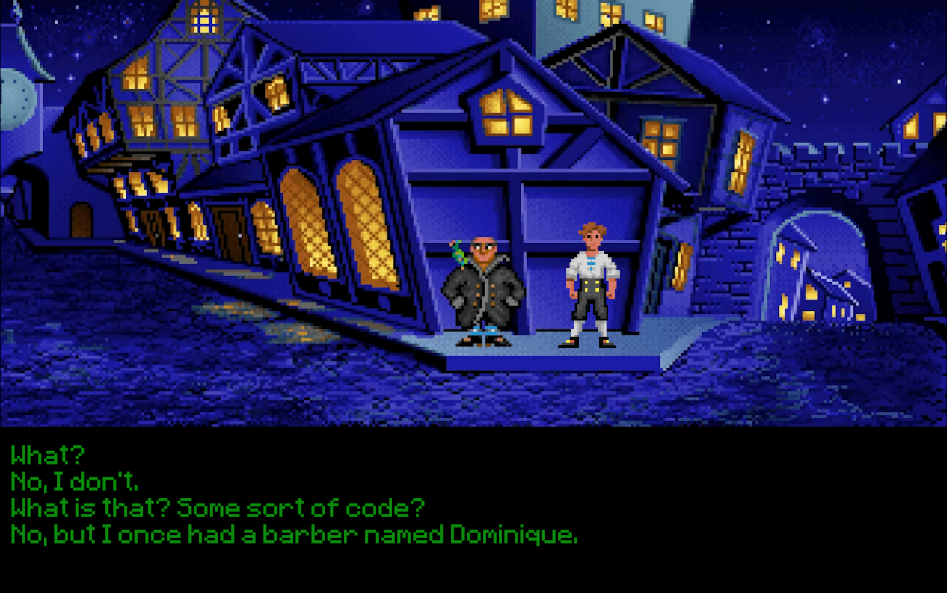
\includegraphics[width=.85\linewidth]{img/User doc/manual-tsomi.png}
\caption{The Secret of Monkey Island (showcase): Dialogue.}
\label{fig:TSoM-manual2}
\end{figure}


\section{Tutorial}
In this section, we will walk the user through creating a scene in the framework like the showcasing ones described in the section above. 

\subsection{Project Setup}
To set up the TaleCraft framework in Unity, the first step is to download and install Unity Hub, following the instructions provided on Unity’s official website at \href{https://unity.com/download}{https://unity.com/download}. Once Unity Hub is installed, the next step is to install Unity Engine version \textbf{2022.3.61f}, which is required to run the project. With the engine in place, the project can be obtained by cloning the repository from GitHub using the following URL: \href{https://github.com/bethkux/TaleCraft}{\textit{https://github.com/bethkux/TaleCraft}}. After the repository has been successfully cloned to a local directory, the project can be opened in Unity Hub by selecting \textbf{Add > Add project from disk} and navigating to the corresponding folder. When the project finishes loading, TaleCraft is ready to use.

Typical point-and-click adventure games often switch between different locations, allowing the player to explore the in-game world. The TaleCraft framework supports this approach by allowing locations to be distributed across multiple scenes. Several systems have been designed with this in mind, including the inventory, which needs to persist between scenes. 

However, for smaller-scale games, switching between scenes that only contain a few dozen \texttt{GameObjects} is generally unnecessary. Additionally, since the framework is designed with beginner users in mind, working in a single scene may be more approachable and less error-prone. As demonstrated by the included showcase games, it is possible to simulate smooth transitions between seemingly separate locations while staying in a single scene.

For these reasons, we recommend that you start by working in just one scene. TaleCraft provides a template scene that you can use to set up the game. It is located in \texttt{Assets > Resources > Template} and includes the most essential parts of the framework. To create a new scene using this template, go to \texttt{File > New Scene} and select \textit{TaleCraft - Template} from the option (see Figure \ref{fig:Tutorial-template:new}). 

\begin{figure}[H]
\centering
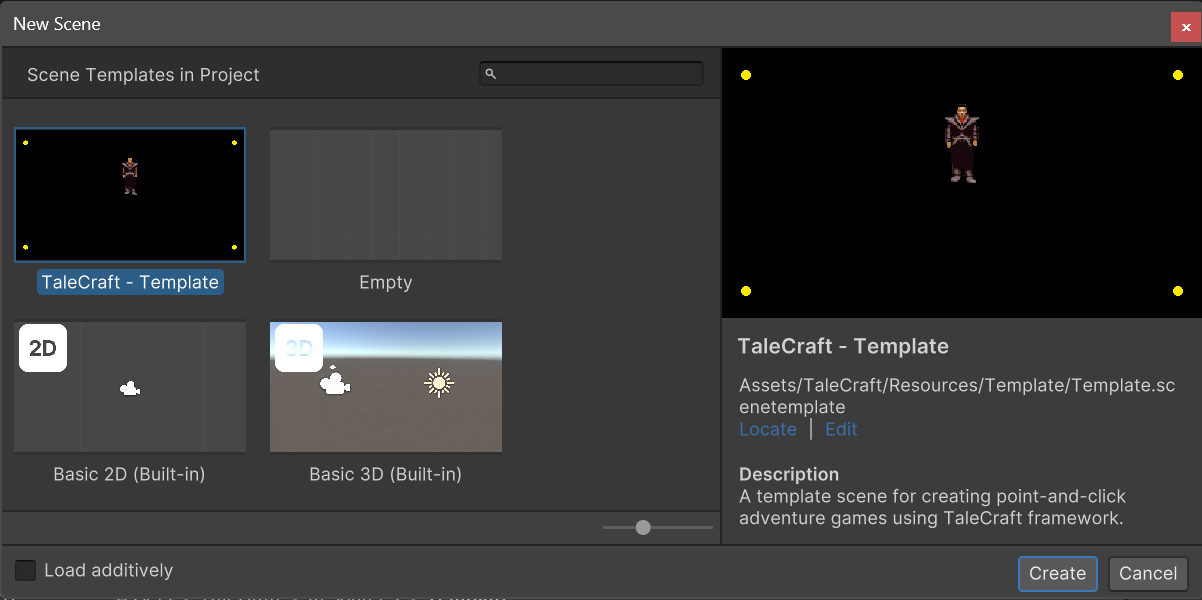
\includegraphics[width=.9\linewidth]{img/User doc/image_2025-07-09_161736255.png}
\caption{Template scene: Creating new scene.}
\label{fig:Tutorial-template:new}
\end{figure}

Figure \ref{fig:Tutorial-template} shows the state of the project when a new template scene is created. On the right is the Scene window, and on the left is the Hierarchy, which lists the \verb|GameObjects| that make up the scene. In the following sections, we will go over the function of some of these objects. For a more structured overview, you can refer to the sections indicated next to each relevant \texttt{GameObject}.

\begin{itemize}
    \item \textbf{PrefabManager} (Section \ref{Manual:Core})
    \item \textbf{CommandManager} (Section \ref{Manual:CM})
    \item \textbf{WalkingSystem} (Section \ref{Manual:WS})
    \item \textbf{EventSystem} (Section \ref{Manual:Core})
    \item \textbf{InputManager} (Section \ref{Manual:Core})
    \item \textbf{SlotManager} (Section \ref{Manual:Core})
    \item \textbf{Canvas}
    \item \textbf{Player} (Sections \ref{Manual:ChM&SS}, \ref{UD-IS})
\end{itemize}

\begin{figure}[H]
\centering
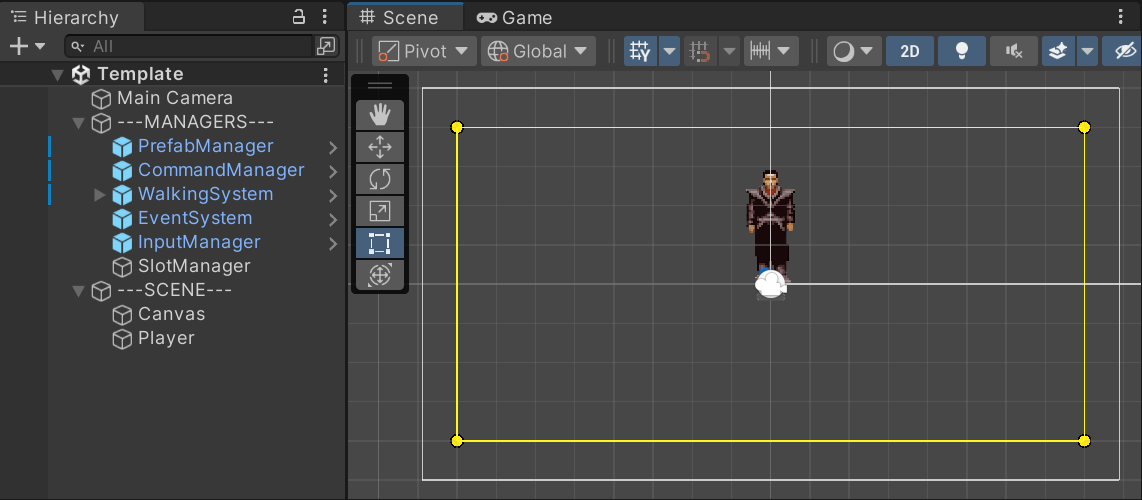
\includegraphics[width=.9\linewidth]{img/User doc/image_2025-07-10_103352984.png}
\caption{Template scene.}
\label{fig:Tutorial-template}
\end{figure}


\subsection{Movement}
The current state of the scene is fairly barebones. However, when starting the game, we can already move the character by clicking inside the yellow rectangle, which marks the walkable area. While it might be tempting to start adjusting this layout right away to fit our vision, our first step will be to add a background.  We add \verb|bg.png|  from the folder \texttt{Assets > TaleCraft > Examples > Scene Assets > Sprites-BaSS > Scene1} by dragging it into the scene. The player might disappear behind the image, but that is okay. All we need to do is adjust the \textit{Order in Layer} in the component \textbf{Sprite Renderer} to a lower number, such as \textit{-99}. Since this is the background and there will be nothing else behind it, we can give it this very low number. The image may not fit into the camera view completely, so let us adjust the scale and position in the \textbf{Sprite Renderer}. Afterwards, the scene should look similar to Figure \ref{fig:Tutorial-template:bg}.
\begin{figure}[H]
\centering
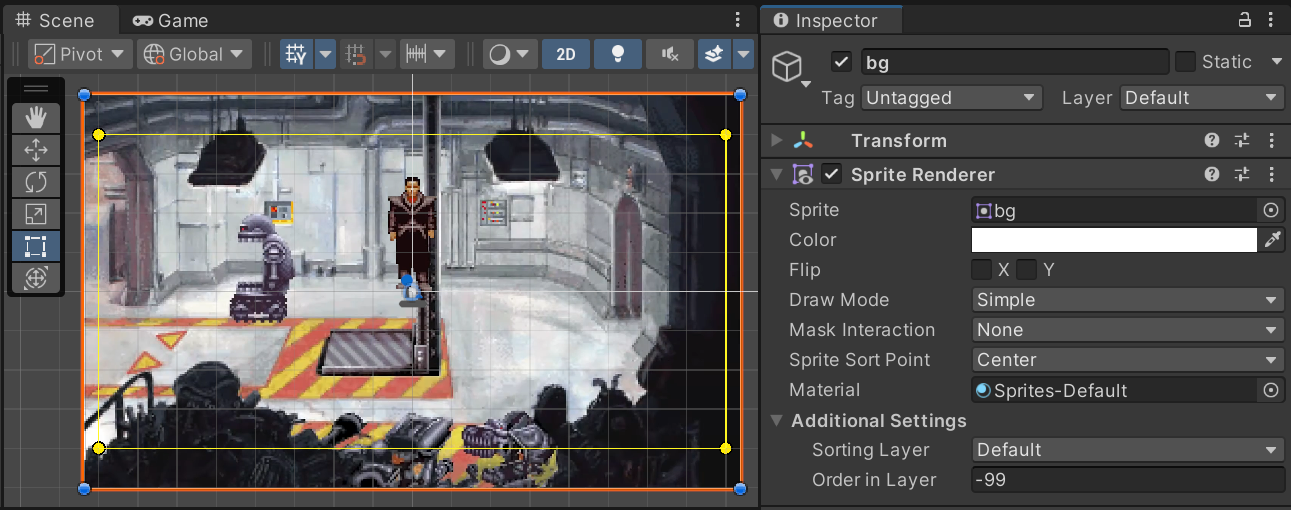
\includegraphics[width=1\linewidth]{img/User doc/image_2025-07-08_104224540.png}
\caption{Template scene: background.}
\label{fig:Tutorial-template:bg}
\end{figure}

Now it is time to adjust the walkable area so that it fits the background and prevents the character from walking on the walls. By clicking on the \verb|GameObject| called \textbf{Main} under \textbf{WalkingSystem} in the hierarchy, handles will appear that make it easy to move the points. Move the points using the handles until the scene looks like Figure \ref{fig:Tutorial-template:main}. To make the area more precise, more points to the polygon can be added by clicking on a white circle in the middle of the line. Details about this system can be found in Section \ref{Manual:WM}.

\begin{figure}[H]
\centering
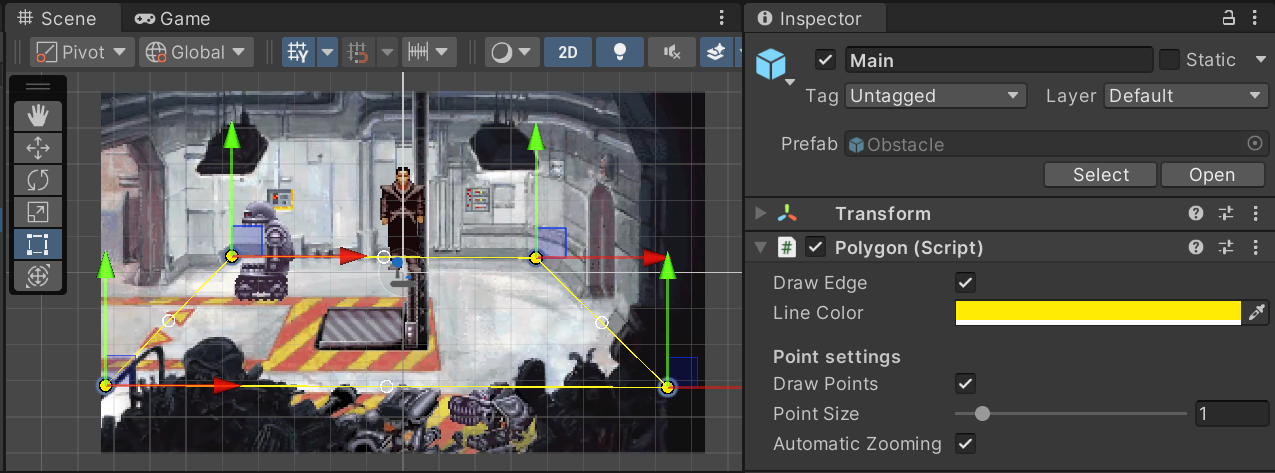
\includegraphics[width=1\linewidth]{img/User doc/image_2025-07-08_104843701.png}
\caption{Template scene: walkable area.}
\label{fig:Tutorial-template:main}
\end{figure}

Now the character moves only on the floor. However, there might occur a situation, when we would like the player to go around an object instead of walking right through it, such as the lift in the middle of the room in our current scene. To do that, we need to create a new obstacle polygon by clicking on button \textit{Build new polygon obstacle} in the inspector of \verb|GameObject| \textbf{WalkingSystem}. The newly generated polygon is too big, so we can modify its layout by selecting the \verb|GameObject| and moving the points. We also recommend changing the color of the polygon in the inspector of the \textbf{Obstacle} polygon for visual clarity. The layout of the lift looks like a trapezoid, but with our five points we have one more than it is needed. We could align the fifth point on the line between two vertices of the trapezoid but a better solution is to remove the point. This is done by holding Ctrl key while clicking on a point (details in Section \ref{Manual:Polygon}). Now the current state of the scene should resemble Figure \ref{fig:Tutorial-template:obstacle}.

\begin{figure}[H]
\centering
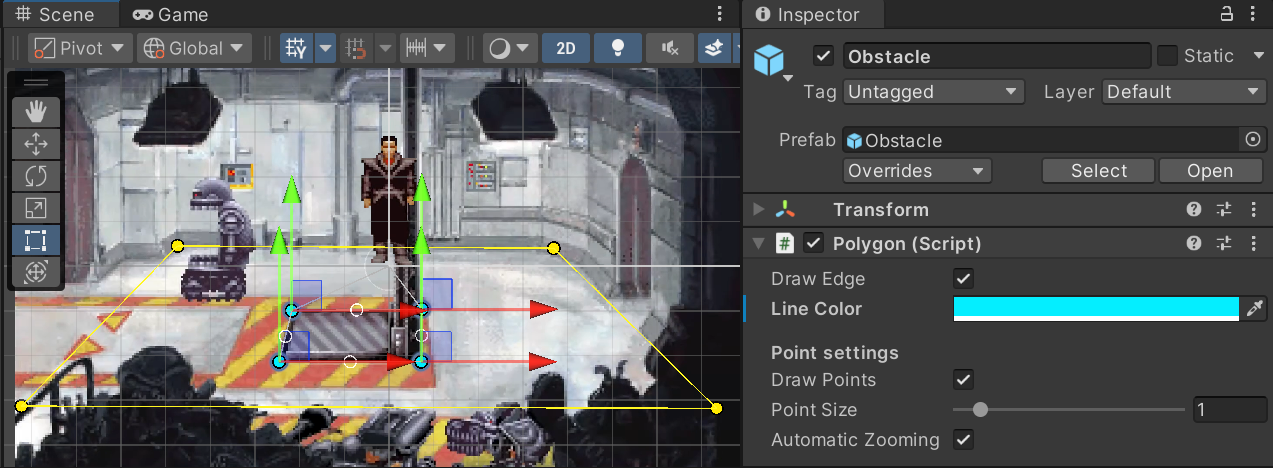
\includegraphics[width=1\linewidth]{img/User doc/image_2025-07-08_110642921.png}
\caption{Template scene: obstacle polygon.}
\label{fig:Tutorial-template:obstacle}
\end{figure}

In this moment we are almost done with the walking system in this scene. When we hit play, we can click around, and the player moves in the main polygon and around the obstacle. The movement is however very slow. To adjust it, we need to click on \textbf{Player} in hierarchy and change the speed in \textbf{Character Movement} component to \textit{2.5}. Now when we run the game, the character moves around more quickly. You might also want to make the character smaller when going into the distance (in this case, to the back of the room). To do that, we can select \textit{Y Scaling} in the \textbf{Sprite Scaler} component. We can already see the sprite of the character change size and the precise scale can be adjusted in the inspector. You can test the character scaling without running the game by simply dragging the character around. Figure \ref{fig:Tutorial-template:Speed&Scaling} shows the current state of the character and the scene. Details about the settings of inspectors with other types of scaling are explained in Section \ref{Manual:ChM&SS}.

\begin{figure}[H]
\centering
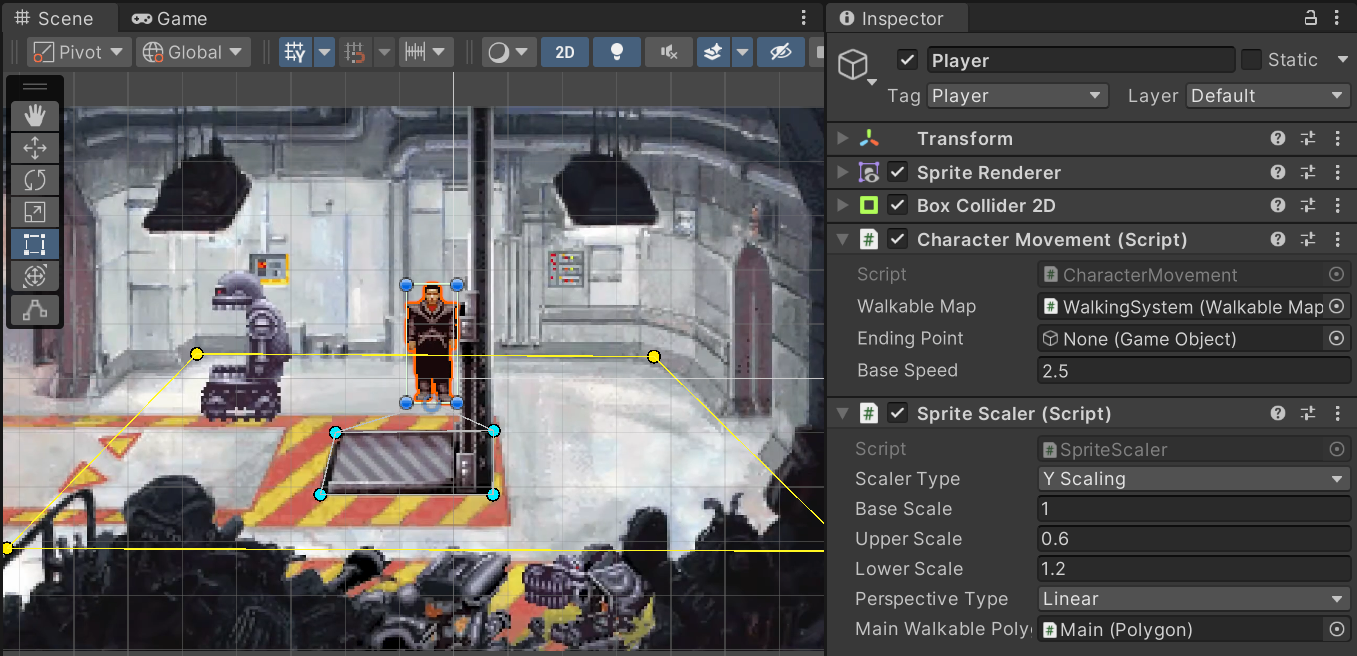
\includegraphics[width=1\linewidth]{img/User doc/image_2025-07-08_111936005.png}
\caption{Template scene: speed and scaling.}
\label{fig:Tutorial-template:Speed&Scaling}
\end{figure}

\subsection{Commands}
Now that we have the movement of the character set up, we can move onto setting up the control system for the player. When selecting the \textbf{CommandManager} in the hierarchy, one command should already be visible: \textit{Command 1}. It is recommended to rename this to something more descriptive, such as \textit{Default}. If the project uses a context-based control system for character interaction, then this setup is already complete. The result should resemble Figure~\ref{fig:Tutorial-template:CM}. However, for command-based games like \textit{The Secret of Monkey Island}, additional commands need to be added. This can be done by pressing the \textit{Add Command} button. After creating the required commands, it is also necessary to define the \textit{Sentence Structure}, which is used to display a short sentence that describes the current action. The complete process of creating new commands and configuring the sentence structure is described in Section~\ref{Manual:CM}.

\begin{figure}[H]
\centering
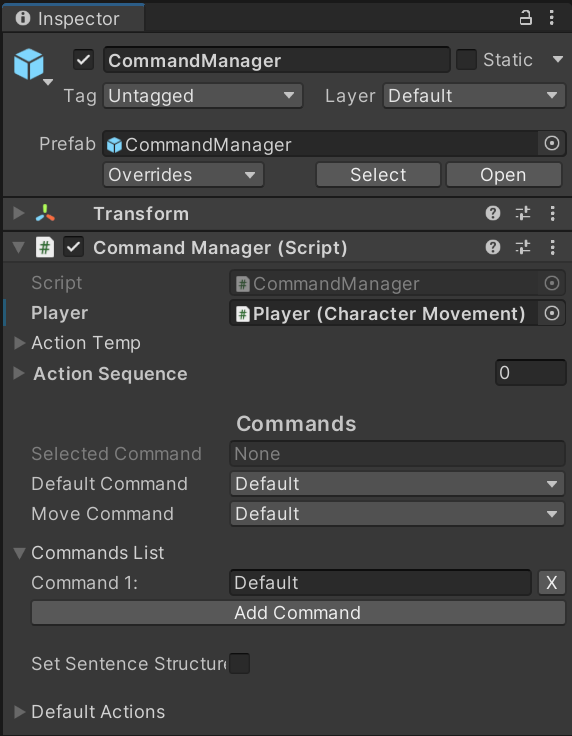
\includegraphics[width=0.6\linewidth]{img/User doc/image_2025-07-08_214350710.png}
\caption{Template scene: Command Manager.}
\label{fig:Tutorial-template:CM}
\end{figure}

Command-based games usually ask the player to pick a command while also showing the action being performed in the form of a sentence (for example, “\verb|Talk to customer|”). To set up the visualization of commands, a new \verb|GameObject| can be created under the \textbf{Canvas} in the hierarchy, with the \textbf{Display Commands} component attached to it. Similarly, to show the current action as a sentence, the \textbf{Display Sentence} component can be added to another \verb|GameObject| under the \textbf{Canvas}. More details about this setup are provided in Section~\ref{Manual:Display-C&S}.

\subsection{World Object}
Now we can move on to creating interactable objects in the scene. A typical point-and-click game includes objects that the player can interact with, be it other characters or simply just regular objects such as a lift. The goal of this section will be to create such an object. Let us start with the large metal robot to the left of the player character. Ideally, this object should not be part of the background, as the background is a static screenshot taken from the original game. Instead, we can place a cutout sprite of the robot on top of the background to achieve the desired visual layering. To do this, locate the sprite named \verb|transporter.png| in the folder \texttt{Assets > TaleCraft > Examples > Scene Assets > Sprites-BaSS > Scene1}, and drag it into the scene. To ensure that the character appears correctly behind the robot when walking, we open the \textbf{Sprite Renderer} component on the robot and set the \textit{Sprite Sort Point} to \textit{Pivot}.

Now we can attach the \textbf{World Object} script as a component to the robot. The first thing we need to do is create a \textbf{World Item} \verb|ScriptableObject| in the Assets folder. This object allows us to set a name and description for the interactable, which is useful not just for displaying tags during gameplay, but also for referencing the object in the editor (see Section \ref{Manual:WO} for more details). In our case, we can use the \texttt{Transporter} object that is already defined under \texttt{Assets > TaleCraft > Examples > BaSS > ScriptableObjects > Items > World > S1} and drag it into the \textit{Item} field of the component.

Next, we can create actions by adding a new element to the \textit{Labeled Actions} list. We can click the \textit{Edit} button to open a new window where we can define what should happen when the object is interacted with. We will return to this point in Section \ref{Manual:Tutorial:D}, when we set up a dialogue. Again, more details about this feature can be found in Section \ref{Manual:WO}.

To specify the exact spot where the character should walk to when interacting with the robot, we can add a \textit{Go To} point in the list shown in the inspector. This helps ensure that the character reaches the right position before the action is executed. Let us set one with a vector \texttt{(0, -0.5)}.

At this point, when we run the game and click on the place where the robot is located, it will still not respond to clicks. To fix this, we need to add a 2D collider so the object can detect mouse interaction. For this type of object, we recommend using a \textbf{Box Collider 2D}. After completing this setup, the inspector should resemble Figure \ref{fig:Tutorial-template:WO}, and clicking on the robot while the game is running should cause the character to walk to the designated spot and perform the assigned action.

\begin{figure}[H]
\centering
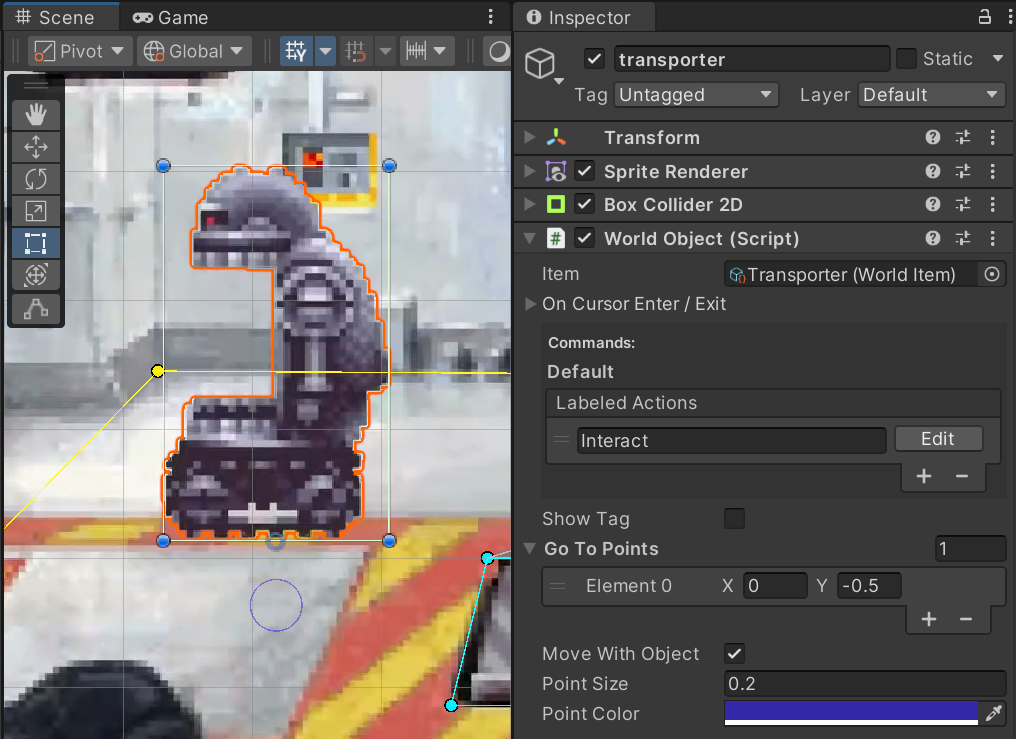
\includegraphics[width=0.8\linewidth]{img/User doc/image_2025-07-08_120956206.png}
\caption{Template scene: World Object.}
\label{fig:Tutorial-template:WO}
\end{figure}

\subsection{Inventory Object} 
So far, we learned how to create objects that the player can interact with. Point-and-click adventure games often put a heavy emphasis on items not only in the environment but also in the inventory. Next step is setting up the other type of interactables: \textbf{Inventory Objects}. Similar to \textbf{World Object}, an Inventory Object also needs a \verb|ScriptableObject|, in this case \textbf{Inventory Item}. The asset contains not only a name and a description box, but also a way to reference a sprite for displaying an icon in the inventory if needed. For our tutorial, we will use one from the already created under \texttt{Assets > TaleCraft > Examples > BaSS > ScriptableObjects > Inventory > World > S1}, but to create and set up a new one follow instructions in \ref{Manual:IO}.

The \textbf{InventorySlot} is a prefab located in the \texttt{Assets > TaleCraft > Prefabs} folder and already includes several useful components, such as the \textbf{Inventory Object} component. To preserve this prefab as a base template, it is recommended to create a \textit{Prefab Variant} by right-clicking on it and selecting the appropriate option. What we are mainly interested in at this point is setting up the desired \textit{Event Types} under the \textbf{Event Trigger} component and assigning the corresponding actions using the \textbf{Custom Pointer Handler} and \textbf{Trigger Setter} components. These tools help define how the slot responds to input events such as clicks and drags. For the purpose of this tutorial, we will not configure these manually, as we will be using a preconfigured prefab in the next steps. More information about these components can be found in Section \ref{Manual:IO}.


\subsection{Inventory}
Now let us create an inventory. It consists of two main parts: the controller and the visualizer. The controller is handled by the \textbf{Inventory Manager}, while the visualizer is set up through the \textbf{Display Inventory} component.

The \textbf{Inventory Manager} is already present in the \textbf{Player} \verb|GameObject|. This is where \texttt{Inventory Items} can be assigned so that they appear in the inventory during gameplay. To do this, press the \texttt{+} button in the inspector and assign the item \verb|MetalBar| from \texttt{Assets > TaleCraft > Examples > BaSS > ScriptableObjects > Items > Inventory} to the new entry (see Figure \ref{fig:Tutorial-template:IM}).

\begin{figure}[H]
\centering
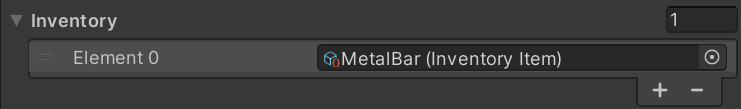
\includegraphics[width=0.7\linewidth]{img/User doc/image_2025-07-10_135818202.png}
\caption{Template scene: Inventory Manager.}
\label{fig:Tutorial-template:IM}
\end{figure}

We have the backend of our inventory working, so now we set up the visual part of the inventory using the \textbf{Display Inventory} component. We create a new \verb|GameObject| under the \textbf{Canvas} in the hierarchy and attach the component to it. Then, we can assign the \textbf{Inventory Manager} we want to use by dragging the \textbf{Player} \verb|GameObject| from the hierarchy into the corresponding field, since it already contains the Inventory Manager.

The component also requires a reference to the \texttt{Inventory Slot} prefab. For the purpose of this tutorial, we will use a prefab from \texttt{Assets > TaleCraft > Examples > BaSS > Prefabs} called \texttt{InventorySlot-BaSS}, which already has some actions configured. There is one more thing that we need to do. In the hierarchy, we need to create a \textbf{TagManager} \texttt{GameObject}, which will come in handy shortly. We add component \textbf{Tag Manager} to it and set it up according to Figure \ref{fig:Tutorial-template:TM}. 

\begin{figure}[H]
\centering
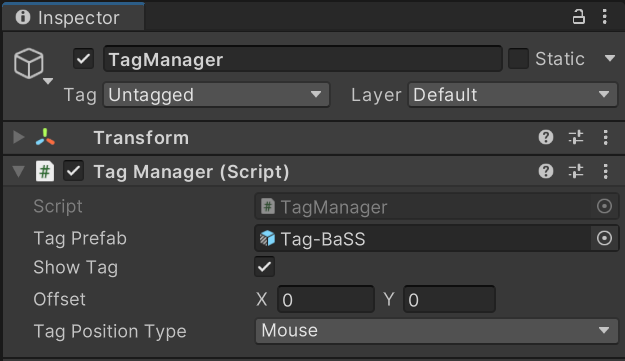
\includegraphics[width=0.6\linewidth]{img/User doc/image_2025-07-09_135233837.png}
\caption{Template scene: Tag Manager.}
\label{fig:Tutorial-template:TM}
\end{figure}

Additionally, we can choose whether the inventory should be text-based or icon-based, configure the layout, and set the maximum number of items allowed.

Once everything is set up and the game is running, we should see an inventory slot displayed on the screen, as shown in Figure \ref{fig:Tutorial-template:Inv}. When we hover over the inventory slot, we get a tag and clicking on the slot with left mouse button displays a description of the item.

\begin{figure}[H]
\centering
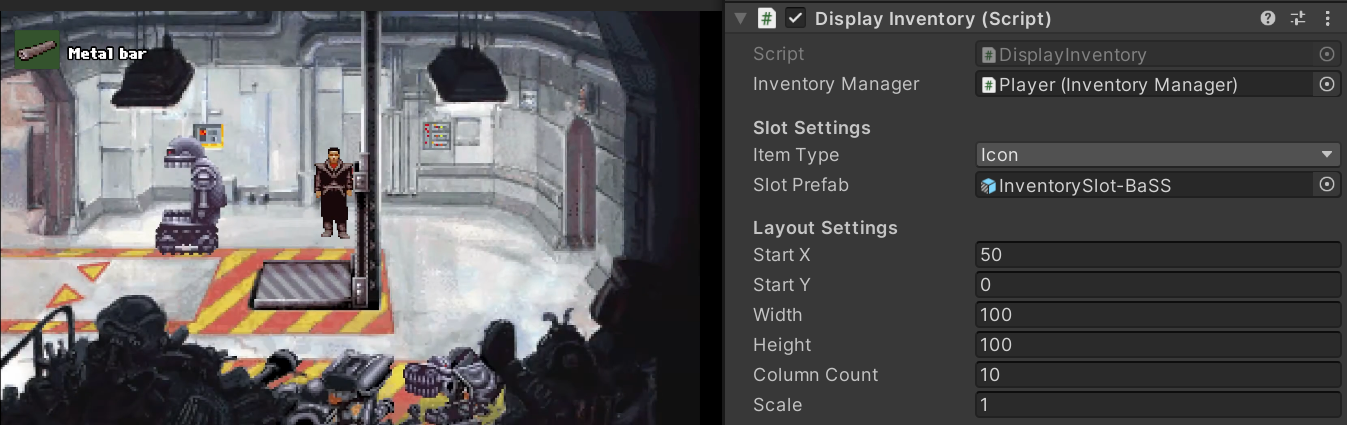
\includegraphics[width=1\linewidth]{img/User doc/image_2025-07-09_135900005.png}
\caption{Template scene: Inventory.}
\label{fig:Tutorial-template:Inv}
\end{figure}

A key action when working with an inventory is adding or removing items. This process is straightforward. Since the framework's command system uses Unity Events, we can reference the \textbf{Inventory Manager} on the \textbf{Player} \texttt{GameObject} by dragging it into the empty field. Then, we choose the action we want, either \texttt{InventoryManager.AddItem} or \texttt{InventoryManager.RemoveItem}. These functions require us to specify which item to add or remove, and we do this by dragging the appropriate \textbf{Inventory Item} asset into the field. Once set up, the inventory will automatically update and display the new state, as shown in Figure \ref{fig:Tutorial-template:InvAdd}.

\begin{figure}[H]
\centering
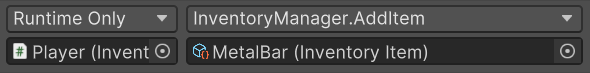
\includegraphics[width=0.7\linewidth]{img/User doc/image_2025-07-10_135422445.png}
\caption{Template scene: Adding items into the inventory.}
\label{fig:Tutorial-template:InvAdd}
\end{figure}

\subsection{Dialogue}
\label{Manual:Tutorial:D}
Now we are ready to move onto the final step of creating a scene -- setting up a conversation. The first step is to create a \texttt{CharacterID} asset for each character the player will interact with, including the player character (see Section \ref{Manual:DS}). This \texttt{ScriptableObject} allows us to set a name and an offset, which will become important shortly.

Next, we need a way to represent a dialogue. For that, we use a dialogue graph asset. Since the detailed process of building a graph is covered in Section~\ref{Manual:DS}, we will not describe it in detail here. However, it is important to note how the \texttt{CharacterID} is used in this process. In the dialogue graph, we can reference a \texttt{CharacterID} to assign specific lines of dialogue to a character. To actually link the characters in the scene with the dialogue system, we use the \textbf{Dialogue Controller} component. We can use a prefab from the Assets of our framework by dragging \textbf{DialogueController} from \texttt{Assets > TaleCraft > Prefabs} into the hierarchy under \textbf{Canvas}. In the inspector, there is a list of pairs: one for the \texttt{CharacterID} and one for the corresponding \texttt{GameObject}. This is where the actual connection is made. For example, to set up the player character, we can add a new element by pressing the + button, drag the \textbf{Player} \texttt{GameObject} into the field labeled \textit{Character} and assign the appropriate \texttt{CharacterID} asset to the field labeled \textit{ID}. In this case, the \texttt{CharacterID} for \textbf{Foster} can be found under \texttt{Assets > TaleCraft > Examples > BaSS > ScriptableObjects > Characters}. The list in the inspector should look like Figure \ref{fig:Tutorial-template:DC}.

Now, there are two more tools under the list. They are both Unity Events and they execute actions before and after the conversation begins or ends. Let us say that when the player starts a conversation, we do not want them to look through the inventory or interact with other \texttt{GameObjects}. On the other hand, when the conversation ends, we need to give control back to the player. We can achieve that using these two Unity Events. For this tutorial, let us say that we do not want the player to move around. So we will create a new entry in both Unity Events, drag the \textbf{Player} \texttt{GameObject} into the field and select \texttt{CharacterMovement.enabled} function. For the first one, we set it to false and for the second one to true. The inspector should resemble Figure \ref{fig:Tutorial-template:DC}.

\begin{figure}[H]
\centering
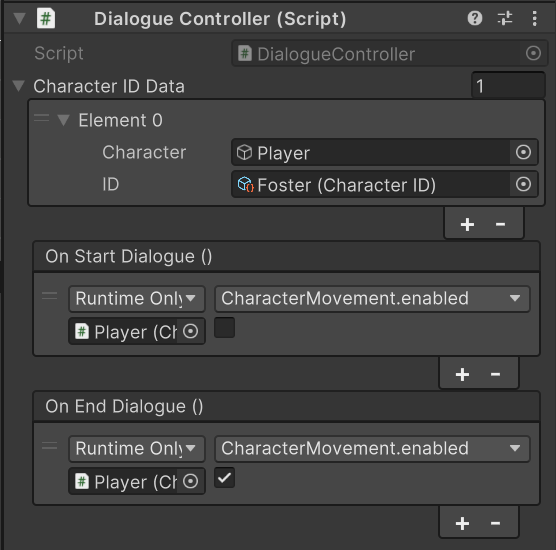
\includegraphics[width=0.6\linewidth]{img/User doc/image_2025-07-09_104007947.png}
\caption{Template scene: Dialogue Controller.}
\label{fig:Tutorial-template:DC}
\end{figure}

You may have noticed that the \texttt{DialogueController} \texttt{GameObject} also contains the \textbf{UI Dialogue Controller} component. There is no need to modify this component at the moment, as everything is already configured and ready to use. For more details about this component, refer to Section~\ref{Manual:DS}.

Now we are ready to run the dialogue. Begin by selecting the \texttt{transporter} \texttt{GameObject} that we set up earlier. Next, we will modify one of the actions in the \textit{Labeled Actions} list by clicking the \textit{Edit} button. A new window will appear, allowing us to set up conditions and previous interactables. We will not focus on those settings now. To learn more about them, refer to Section~\ref{Manual:WO}. Instead, we will concentrate on the section below. In the \textit{Duplicate Actions} area, there should be a single option available: \textit{Move Closer} and a Unity Event. Enable \textit{Move Closer} by checking the corresponding box, and then add a new Unity Event. We want to reference the \texttt{DialogueController} from the scene, so let us drag the \texttt{GameObject} into the empty object field of the Unity Event. Once the reference is set, we choose the function \texttt{DialogueController.StartDialogue}. This function takes one parameter: the Dialogue Graph Data. We will use an existing asset found under \texttt{Assets > TaleCraft > Examples > BaSS > ScriptableObjects > Graphs > InteractGraphs > S1} named \textbf{Transporter\_I}. After assigning the asset, the window should look like Figure~\ref{fig:Tutorial-template:AW+DC}.

\begin{figure}[H]
\centering
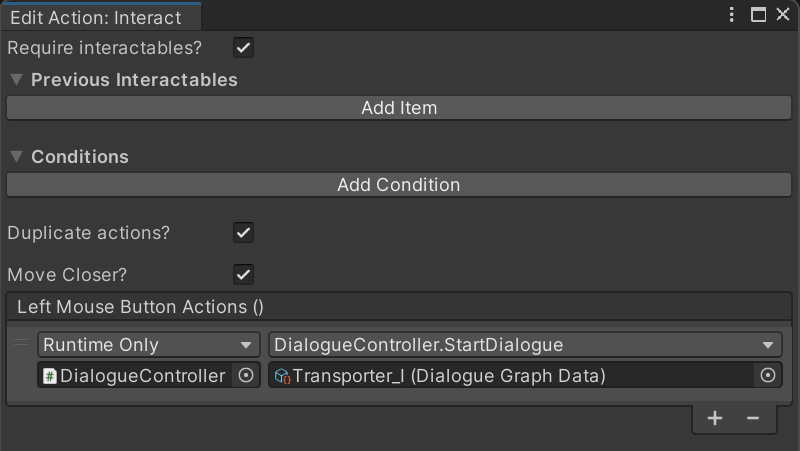
\includegraphics[width=0.75\linewidth]{img/User doc/image_2025-07-09_112421422.png}
\caption{Template scene: Action window with Dialogue Controller.}
\label{fig:Tutorial-template:AW+DC}
\end{figure}

Now when we close the window and run the game, by clicking on the robot the character will move closer to it and a sentence will appear above the head of the character, just like in Figure \ref{fig:Tutorial-template:fin}.

\begin{figure}[H]
\centering
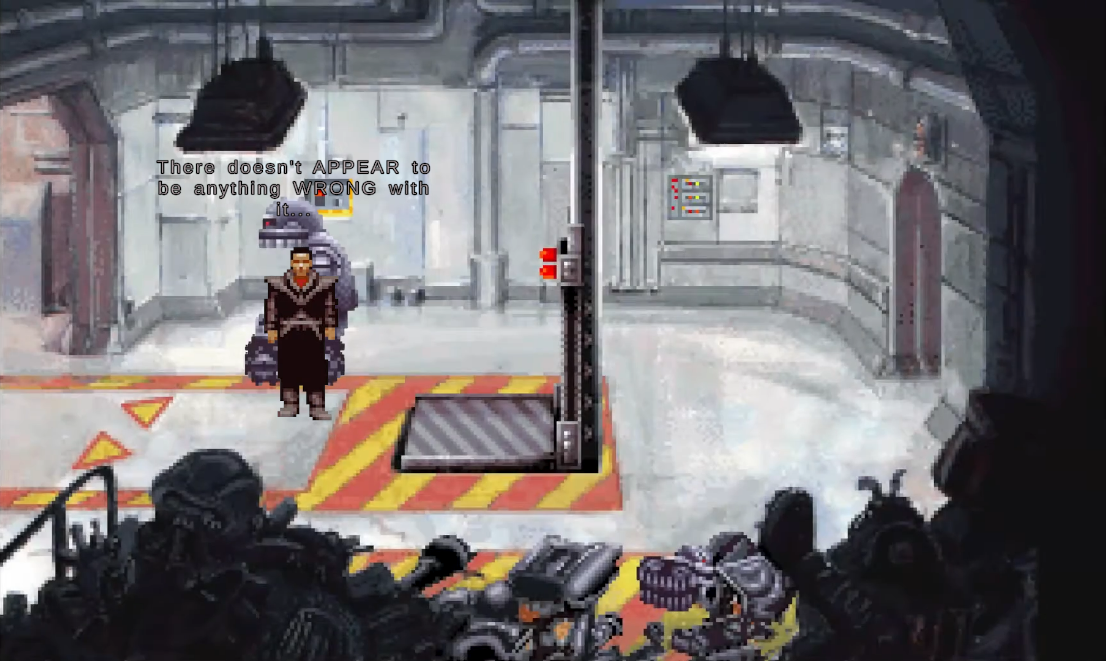
\includegraphics[width=0.85\linewidth]{img/User doc/manual-fin.png}
\caption{Template scene: Conversation.}
\label{fig:Tutorial-template:fin}
\end{figure}

\subsection{Conclusion}
You can save your newly created scene by going to \texttt{File > Save} in the top toolbar. Choose a location in the \texttt{Assets} folder to store it. We recommend saving it outside the \texttt{TaleCraft} folder to keep a clear separation between the framework and your own project files.


\section{Framework}
The TaleCraft framework consists of five main systems whose role is to manage and execute the primary features of a point-and-click adventure game. We will go through each of them and explain the ideal process of creating a game using this framework. The project also includes two scenes that showcase the use of our framework and are located under \verb|Assets > Examples|. In this chapter, we will refer to these two scenes by an abbreviation. The scene from our framework showcasing an area from \textit{Beneath a Steel Sky} (1994) will be referred to as \textit{BaSS}, whereas the one from \textit{The Secret of Monkey Island} (1990) will be called \textit{TSoMI}.

\subsection{Core}
\label{Manual:Core}
To create a scene using the TaleCraft framework, it must include a \verb|GameObject| with the \textbf{Prefab Manager} component. This component provides a centralized and convenient way to reference prefabs across the framework's scripts. The Prefab Manager relies on a \verb|ScriptableObject| called the \textbf{Prefab Library}, which stores a dictionary of prefabs accessible via string labels. A new Prefab Library asset can be created in the \verb|Assets| folder by right-clicking and selecting \verb|Create > Prefab Library|.

Multiple parts of the framework make use of the Prefab Library to instantiate or reference prefabs. The \verb|Assets/Prefabs| directory contains an instance of the Prefab Library, along with a collection of predefined prefabs tailored for the framework. These prefabs are already referenced within the Prefab Library and are intended to be reused and extended by users of the framework.

For the game to process input from the player, a scene also needs to include two other \verb|GameObjects|: \textbf{Event System} and \textbf{Input Manager}. They are both located under Prefabs in the framework \verb|Assets| folder and can be put into the scene by simply dragging the prefab into the hierarchy. \textbf{Event System}'s role is to send events to objects in the application based on input (e.g. keyboard, mouse), while \textbf{Input Manager} processes the input with the help of Player Input component. For users trying to set up specialized behavior for certain inputs can do so using this input system.

The final script in the Core system is \textbf{Cursor Locker}, which is used on many occasions in this framework. Game designers typically do not want the player to interact with objects on the scene during cutscenes or during dialogue, so this script helps manage it. It is an optional script and can be included into the project as a component if you need to manage the behavior of the cursor. To use its functionality in Unity Events for example (depicted in Figure \ref{fig:Manual-UnityEvents}), you needs to drag the \verb|GameObject| with the \textbf{Cursor Locker} component into the row and then select the appropriate function.


\begin{figure}[H]
\centering
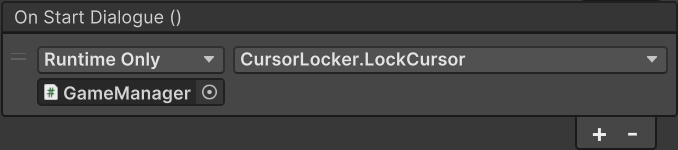
\includegraphics[width=0.7\linewidth]{img/User doc/image_2025-07-09_124713377.png}
\caption{Calling function using Unity Events.}
\label{fig:Manual-UnityEvents}
\end{figure}


\subsection{Walking System}
\label{Manual:WS}
The walking system is a good starting point right after setting up the the core system. 

\subsubsection{Walkable Map}
\label{Manual:WM}
The framework provides its own default implementation of the prefab which contains a \verb|GameObject| with \textbf{Walkable Map} script attached to it as a component and by navigating the menu options \verb|GameObject > Walking System| it can be instantiated in the hierarchy. The prefab also comes with a polygon that describes the walkable area accessible to characters. In Figure \ref{fig:Manual-WM}, we can see Unity inspector for the \textbf{Walkable Map} component together with a possible use of this component in scene \textit{BaSS}. An important part of the walking system is the possibility to create obstacles for the player. To do that, you can simply press at the \textit{Build new polygon obstacle} button, which generates a new \verb|GameObject| with the \textbf{Polygon} component script attached to it (see Figure\ref{fig:Manual-Polygon}). To remove this obstacle from the walking system, one can simply press the button \textit{X} next to the desired polygon in the list of obstacle polygons. 

\begin{figure}[H]
\centering
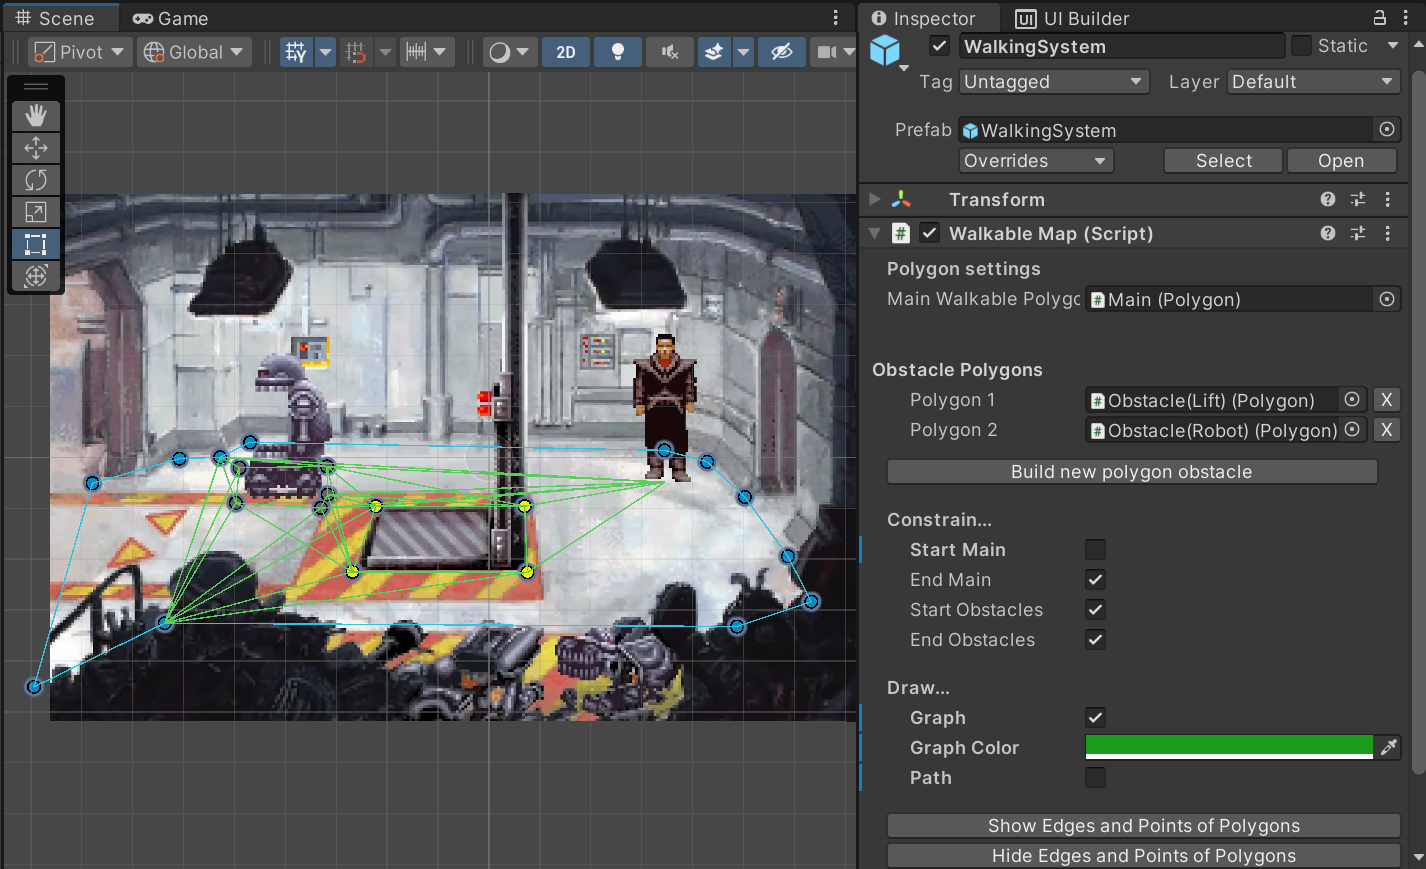
\includegraphics[width=1\linewidth]{img/User doc/walkable_map.png}
\caption{Walkable Map inspector.}
\label{fig:Manual-WM}
\end{figure}

Below that, there are options to constrain the starting or ending points inside the walkable area and outside the obstacle polygons. In other words, if the player clicks on a point outside the walkable area defined by the developer and the option \textit{End Main} is true, then the system will find the closest possible point in the walkable area from the position of the mouse and will move the character to that point. On the other hand, if false is selected, the character will not move as there is no possible path to the position of the mouse click. Similar rules apply to the \textit{End Obstacles} option, where if a mouse click is registered to be inside an obstacle polygon, the closest possible accessible position is found in the walkable area. The \textit{Start Main} and \textit{Start Obstacle} options work similarly but for the starting position, meaning the character. If the character finds itself to be outside the walkable area and the option \textit{Start Main} or \textit{Start Obstacles} is selected, the character will try to find a way to the given position, otherwise not.

Finally, the component also contains some visual enhancements for the developer. It is possible to visualize the graph created by the polygons and the character with the option to select the desired color for the graph. At the bottom, there is an option to quickly show or hide all edges and points of all polygons contained in this walking system. 

\subsubsection{Polygon}
\label{Manual:Polygon}
The Figure \ref{fig:Manual-Polygon} shows an example of an obstacle polygon. The inspector provides some basic visual tools to help the workflow. These settings include the visibility of the edges and points together with a color that can be set easily to visually distinguish different polygons from one another. One option also includes the sizing of the points together with the possibility to turn off automatic zooming. \textit{Automatic zooming} (depicted in Figure \ref{fig:Manual-Zoom}) makes the points change size based on the zoom level of the scene. If turned off and zoomed in, the points become very large and the screen is unreadable, so this option is turned on by default.

Undoubtedly, a developer needs to adjust the position and the number of nodes. When the given polygon is selected in the hierarchy, the position handles can be seen on top of the vertices of the polygons. These enable easy and intuitive editing of points without the need to individually click on each point \verb|GameObject| in the hierarchy. If you then wish to add a new point, simply click on the circle in the middle of the line between two already present points. A new point \verb|GameObject| with the component \textbf{Point} is then created in the exact position of the circle. If a point needs to be deleted, you need to press the Ctrl key and click on the given point. If done so, the point is removed and a new line edge is formed between the two neighboring points.
\begin{figure}[H]
\centering
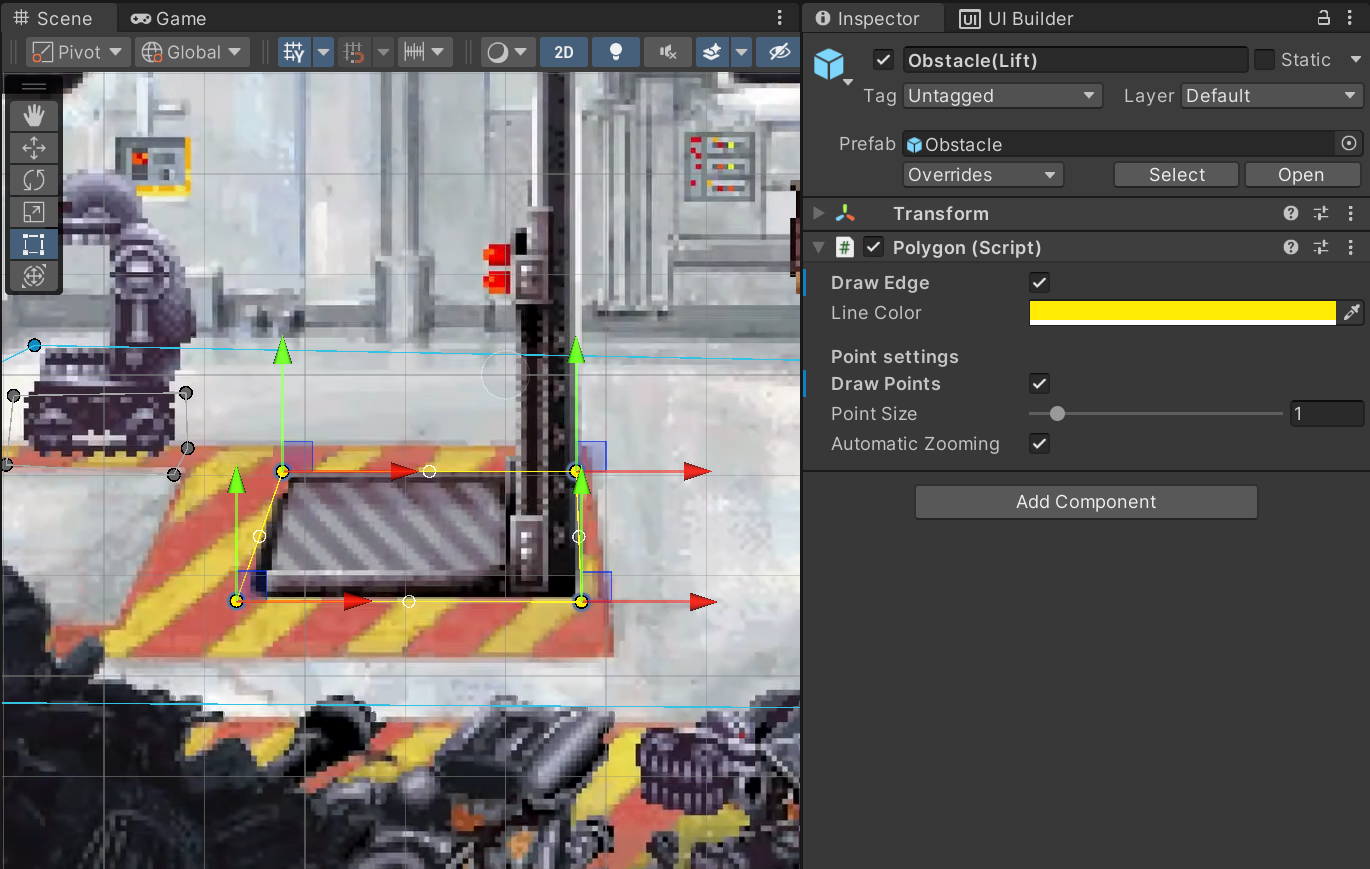
\includegraphics[width=1\linewidth]{img/User doc/polygon.png}
\caption{Polygon inspector.}
\label{fig:Manual-Polygon}
\end{figure}

\begin{figure}[H]
\centering
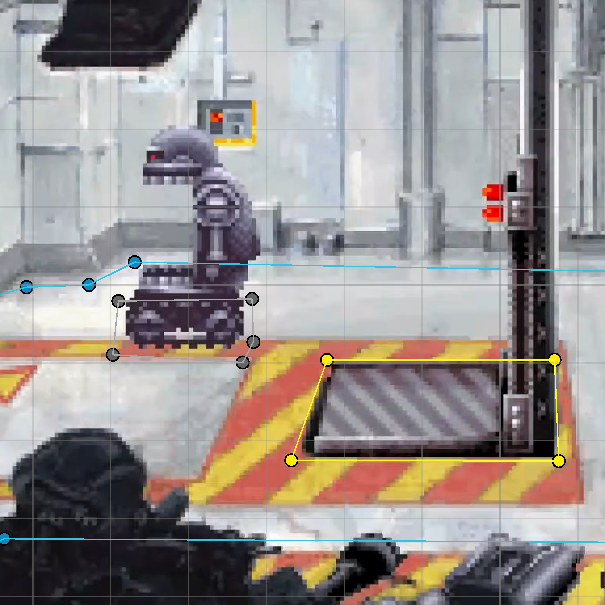
\includegraphics[width=.48\linewidth]{img/User doc/point_scaling.png}
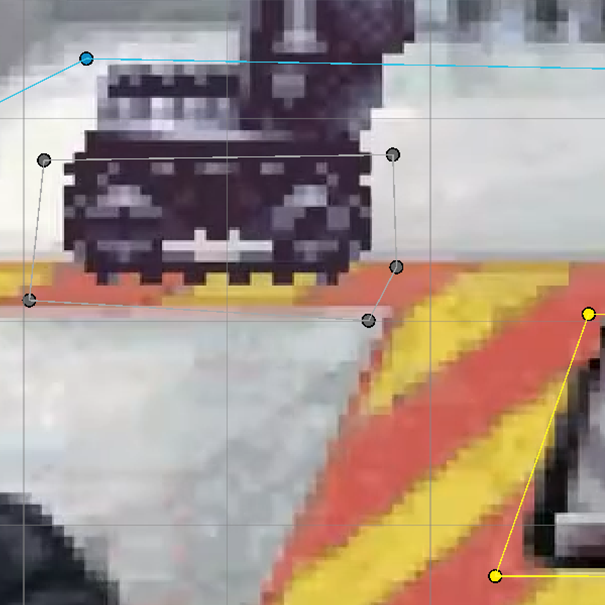
\includegraphics[width=.48\linewidth]{img/User doc/point_scaling2.png}
\caption{Point scaling based on zoom level.}
\label{fig:Manual-Zoom}
\end{figure}

\subsubsection{Character Movement \& Sprite Scaler}
\label{Manual:ChM&SS}
The last two components of the walking system are \textbf{Character Movement} and \textbf{Sprite Scaler} scripts, whose application in the framework can be clearly seen in Figure \ref{fig:Manual-ChM&SS} for scene \textit{TSoMI}. 

\begin{figure}[H]
\centering
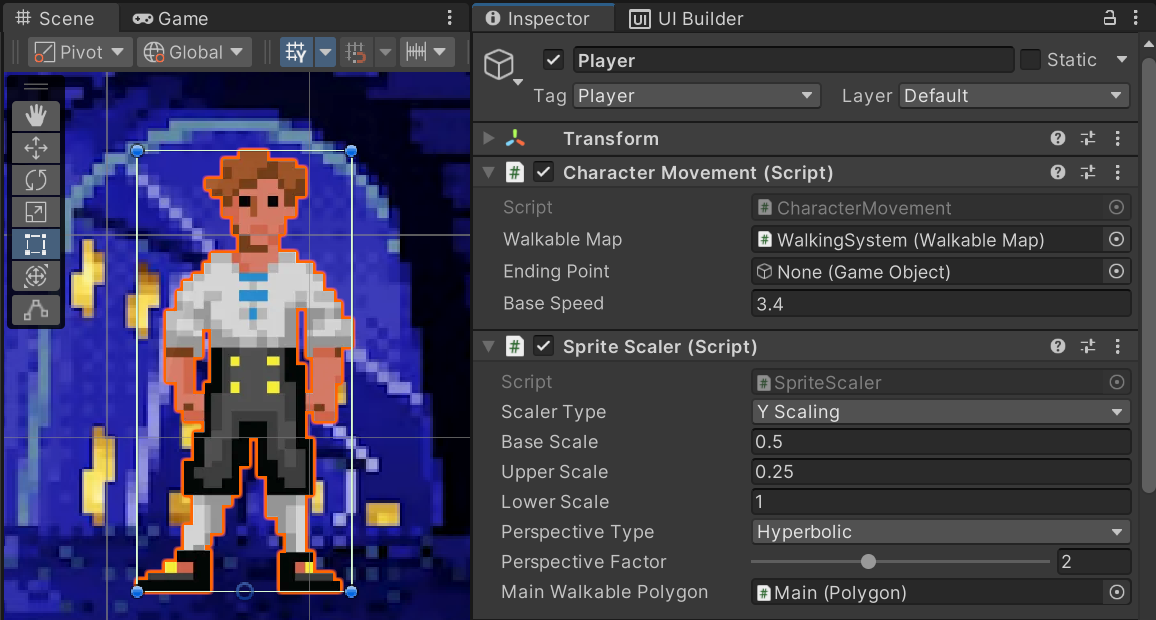
\includegraphics[width=0.9\linewidth]{img/User doc/character_movement.png}
\caption{Character Movement and Sprite Scaler inspector.}
\label{fig:Manual-ChM&SS}
\end{figure}


The \textbf{Character Movement} script is attached to the player \verb|GameObject| or to any other character that requires movement in a walkable area. The script must have a reference to the \textbf{Walkable Map}, and the desired movement speed can be configured. An optional end point may also be specified, primarily for debugging purposes. When defined, the graph in the \textbf{Walkable Map} component can visualize the path between the character's current position and the designated end point without entering play mode. This allows us to interactively reposition the end point and verify that the polygonal navigation areas are configured correctly.

Finally, the \textbf{Sprite Scaler} component takes care of scaling the sprite of the object to which the component is attached. There are multiple options to choose from. The first option is \textit{None}, meaning no scaling is applied to the character. The other two options are \textit{X }and \textit{Y-based scaling}, where the scaling occurs based on the X or Y axis. The two borderline cases need to be selected, which define the scale the very top and bottom for Y axis or very left and right for X axis of the walkable area. The type of perspective can be also selected. If the \textit{Linear} option is enabled, the character scales linearly. The \textit{Hyperbolic} option provides more variety with the rate of scaling. The last scaling type is \textit{Custom}, which takes the scaling factor in each point in the component \textbf{Point} of the walkable polygon and interpolates between them based on the distance.

\subsection{Command System}
\label{Manual:CS}
The Command system is complex and contains many components, so let us take a closer look at its individual parts.

\subsubsection{Command Manager}
\label{Manual:CM}
The framework can instantiate a prefab in the hierarchy by navigating the menu options \verb|GameObject > Command System|. The prefab consists of a \verb|GameObject| with \textbf{Command Manager} script attached to it as a component (see an example of  the script from scene \textit{BaSS} in Figure \ref{fig:Manual-CM}). It takes the player \verb|GameObject| as a reference to apply action like walking to the appropriate location. The other two following properties \textit{Action Temp} and \textit{Action Sequence} are for debugging purposes as they display the currently hovered over object and the other \verb|GameObject| that the player has interacted with.

\begin{figure}[H]
\centering
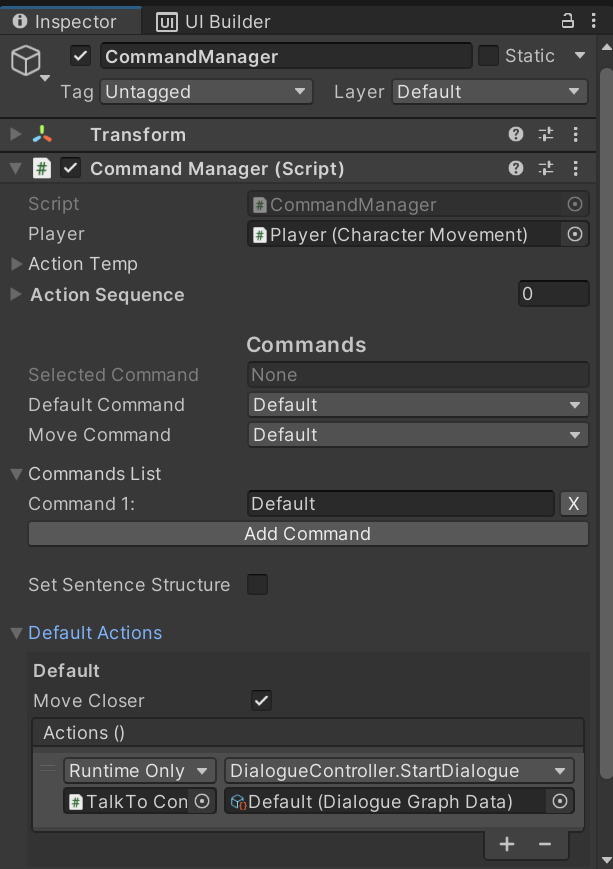
\includegraphics[width=.6\linewidth]{img/User doc/command_manager.png}
\caption{Command Manager inspector.}
\label{fig:Manual-CM}
\end{figure}

The next section, \textit{Commands}, is used to define the behavior associated with each command. All available commands are listed in the \textit{Commands List}. New entries can be added using the \textit{Add Command} button, while existing ones can be removed with the \textit{X} button next to each item. Editing commands in this list will automatically update all references across the framework’s inspectors without data loss. If there is a risk of losing data, the scripts provide separate buttons to synchronize the commands.

Above the list, there is a property displaying the currently selected command, primarily for debugging purposes. Additionally, the section includes options for setting the \textit{Default Command} and the \textit{Move Command}. The \textit{Default Command} determines which command will become active once the current action is completed. On the other hand, the \textit{Move Command} specifies the command responsible for detecting and responding to clicks related to character movement. The scene \textit{TSoMI} can serve as a useful reference for users, as it showcases a variety of commands and highlights the potential of the Command system.

Next is the \textit{Set Sentence Structure} option, which lets you define the structure that the command needs to follow when the command sentence is supposed to be displayed. For example, Figure \ref{fig:Manual-CM3} shows a possible way to set this \textit{Sentence Structures}. “\verb|Talk to|” command is only followed by an object (e.g., “\verb|Talk to customer|”), whereas “\verb|Give|” requires the Object - Connector - Object sequence (e.g., “\verb|Give flower to customer|”).

\begin{figure}[H]
\centering
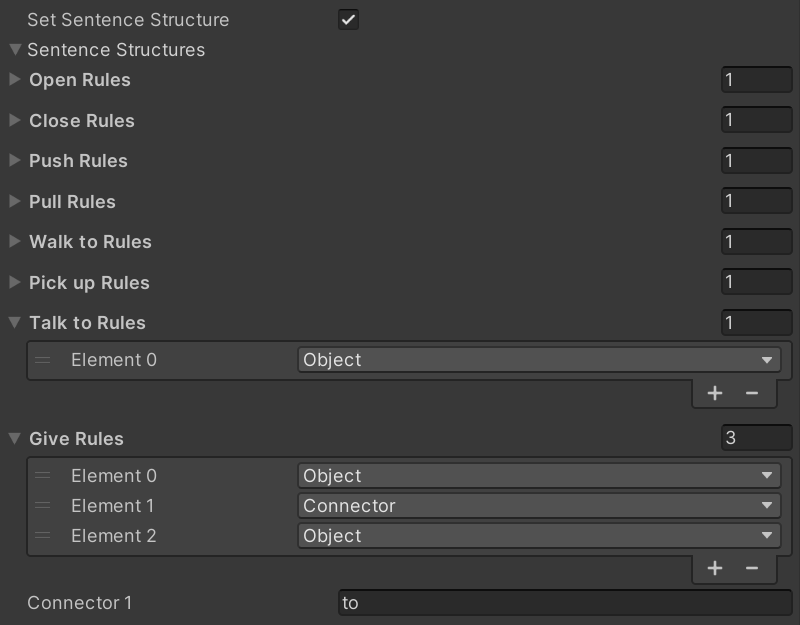
\includegraphics[width=.8\linewidth]{img/User doc/image_2025-07-04_203654317.png}
\caption{Command Manager inspector - Structure.}
\label{fig:Manual-CM3}
\end{figure}

Finally, the \textit{Default Actions} allow us to specify what should happen when all possible actions for a given object-command combination are invalid. This is useful for providing feedback to the player when their input is not correct and a different action is required. If the \textit{Move Closer} toggle is enabled, the character will walk up to the object before attempting to interact with it. The \textit{Actions} section below allows you to define additional behavior through Unity Events.

\subsubsection{Display Command \& Sentence }
\label{Manual:Display-C&S}
The scripts \textbf{Display Command} and \textbf{Display Sentence} allow you to visualize the selection of commands and to present the sentence that represents the currently selected action. The \textbf{Display Command} script is straightforward to configure. In the scene hierarchy under the \textbf{Canvas} object, a new \verb|GameObject| should be created and assigned the \textbf{Display Command} component. Its Inspector window consists of three primary sections: \textit{Layout Settings}, \textit{Used Commands}, and \textit{Unused Commands}.

The \textit{Layout Settings} section manages the visual arrangement of the commands, such as spacing, offset, and positioning. The \textit{Used Commands} section lists the commands currently displayed on screen, while the \textit{Unused Commands} section contains those that are hidden. Initially, all available commands are listed under \textit{Unused Commands}. To display a command, you can click the \textit{+} button beside it, which moves it into the \textit{Used Commands} section. In contrast, commands can be hidden by clicking the \textit{X} button next to a command listed under \textit{Used Commands}. This system allows developers to include additional functionality in the form of commands that is not directly accessible to the player.

The component \textbf{Display Sentence} handles the generation of a sentence that reflects the current command that the player is assembling. The sentence structure is based on the rule set defined in the \textbf{Command Manager} (see Section~\ref{Manual:CM}), where the first word represents the command verb, and subsequent elements are constructed according to predefined grammar rules. The component also supports dynamic positioning of the sentence near the mouse cursor. This behavior can be enabled by toggling the \textit{On Mouse} option, with the exact position adjusted via the \textit{Shift By} property, which accepts a two-dimensional offset vector.

\subsubsection{World Object}
\label{Manual:WO}
In order to set up an interactable object in the scene, you first need to create a \verb|ScriptableObject| in the \verb|Assets| folder by pressing right-click and selecting \verb|Create > Item > World Item|. Here, you can define the name and description of the item. This asset helps to reference the item throughout the whole project, even in other scenes. Features such as the sprite or what the item does when interacted with need to be set in the \verb|GameObject| with the component \textbf{World Object} attached, with a possible implementation in Figure \ref{fig:Manual-WO} from the \textit{BaSS} scene. 

\begin{figure}[H]
\centering
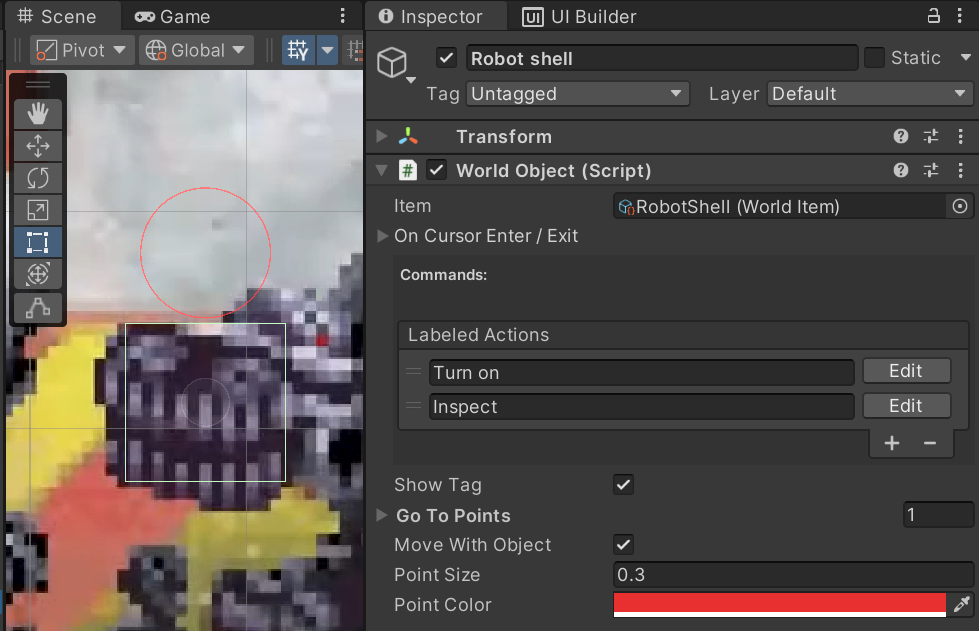
\includegraphics[width=.8\linewidth]{img/User doc/world_object.png}
\caption{World Object inspector.}
\label{fig:Manual-WO}
\end{figure}

The script takes a \textbf{World Item} asset as a reference in order to assign the item with the actions defined. Except for an option to show a tag with a name of the object, the script also offers a way to define the position of the player when interaction is initiated. The can define multiple of these so-called \textit{Go To Points} using 2D vector coordinates and during runtime the closest of them is chosen. If none are defined and the character is ordered to move to that position, it selects the position of the object itself. If the object changes position (it is a moving character, for example), you can define if the position of these points is relative to the object or not. There are also visual tools like selecting a color and the size of the circle defining the point.

The desired behavior can be created in the reorderable \textit{Labeled Actions} list. If the player interacts with the given object, the command system goes one by one in the list and if all required conditions are met, the given action is executed. When creating a new action using the \textit{+} button, you can set a label to that action. This label is purely visual and serves to make the editing of actions readable. When the \textit{Edit} button is pressed, a window pops up, which serves to create the logic of an action. The window first starts with \textit{Previous Interactables}. If enabled, the action is required to contain the same actions as the player had previously interacted with, which can be seen in \textit{Action Sequence} in \textbf{Command Manager}. The next step in verification are \textit{Conditions}, which is a list of \verb|ScriptableObject| \textbf{Variables}, which can be created in the \verb|Assets| folder through the \verb|Create > Variable > ...| option. This lets you define either an integer, a float, a string or a boolean variable. In the action window, the conditions need to be given the expected value. If the \textit{Conditions} or the \textit{Previous Interactables} do not match, the action is considered invalid and the next action in the list is checked. In case everything matches, the \verb|UnityEvents| from the very bottom of the window are called based on the type of the click.

\begin{figure}[H]
\centering
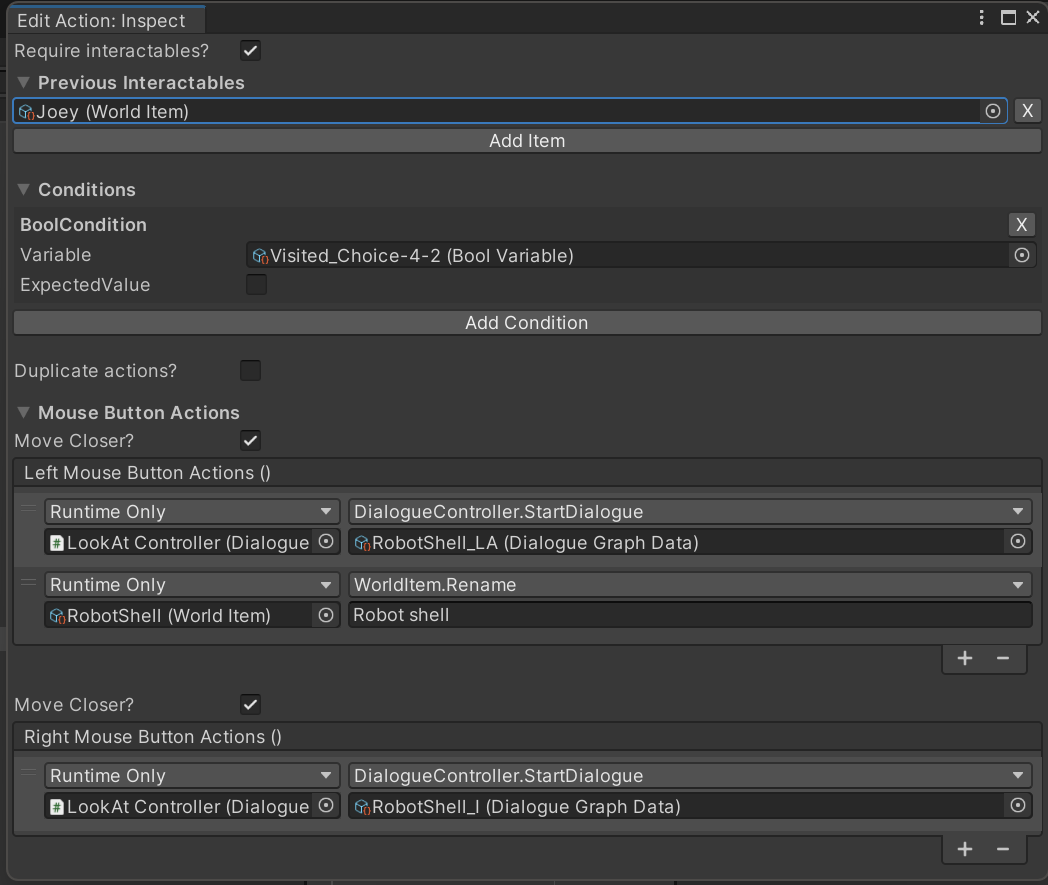
\includegraphics[width=.8\linewidth]{img/User doc/action_window.png}
\caption{Action window.}
\label{fig:BaSS-manual}
\end{figure}

\subsubsection{Inventory Object}
\label{Manual:IO}
\textbf{Inventory Objects} are interactables inside the player's inventory. Unlike \textbf{World Objects}, they cannot be assigned actions that easily, since sometimes the player needs to use an item in another scene and doing so would require you to create a new instance of the same item in every scene. We want to make it easy and intuitive to work with our framework. So we decided to create a \textbf{Slot Manager} in every scene, which would manage the actions of inventory slots in the current scene (see Figure \ref{fig:Manual-SM}). Defining actions is the same as for \textbf{World Objects}, but first we need to create a new slot using the \textit{Add Slot} button. Then, we can to assign the actions to an item using \verb|ScriptableObject| Inventory Item, which can be created by right-clicking in the \verb|Assets| folder and selecting \verb|Create > Item > Inventory Item|. Similar to \textbf{World Item},  we can set the name as well as the description of the item. In addition, there is an option to add a sprite. This feature is used when the inventory is icon-based, more on that in Section \ref{UD-IS}.

\begin{figure}[H]
\centering
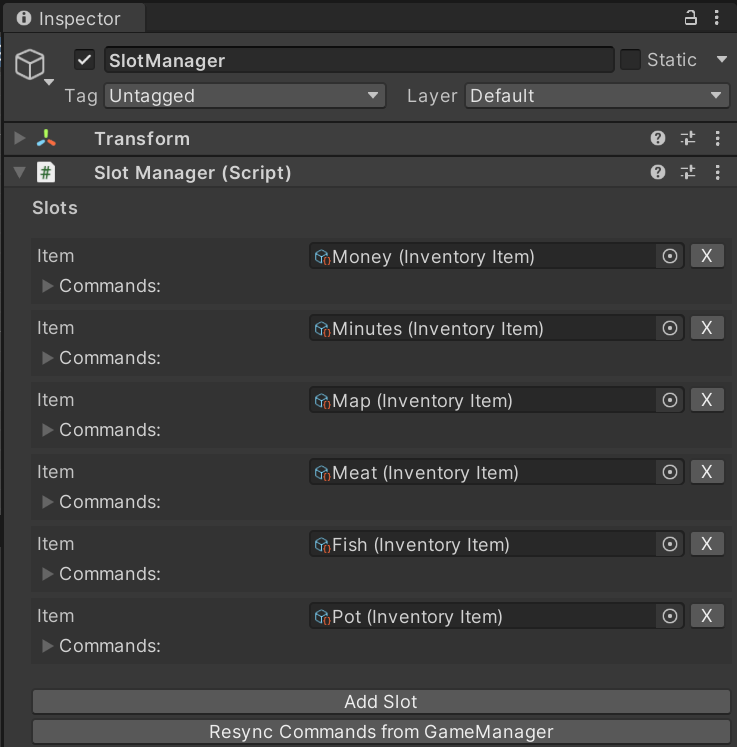
\includegraphics[width=.7\linewidth]{img/image_2025-07-05_133040354.png}
\caption{Slot Manager with six slots for Inventory Items.}
\label{fig:Manual-SM}
\end{figure}

To ensure that an inventory slot appears correctly in the inventory and has expected behaviors, such as being draggable by the mouse cursor or displaying a tag when hovered over, a prefab must be created. This prefab acts as a reusable template, which allows the system to instantiate inventory slot elements automatically, each with the required components and behaviors already configured. Once the prefab is set up properly, we do not need to manually configure each inventory slot instance.

The TaleCraft framework provides a ready-made implementation of such an inventory slot prefab, as demonstrated in the \textit{TSoMI} and \textit{BaSS} example scenes. In order for the framework to access and instantiate this prefab, it must be registered in the \textbf{Prefab Library} under the label \textit{InventorySlot}.

Since inventory slots are part of the user interface (UI), the system for handling input, such as clicking or dragging, differs from that used for \textbf{World Objects}. Moreover, \textbf{World Objects} typically only respond to left or right mouse clicks, whereas inventory interactions may include additional behaviors such as dragging. These behaviors must be defined by the developer, but the TaleCraft framework simplifies the process.

Unity provides the \textbf{Event Trigger} component, which can be attached to a \verb|GameObject| to define responses to various input events, such as cursor entry or exit, clicks, drags, and more. In the TaleCraft framework, inventory slots make use of this system in the provided showcasing scenes \textit{BaSS} and \textit{TSoMI}. In point-and-click games, the player often utilizes both left and right mouse buttons for different action. To help manage that, the framework includes the \textbf{Custom Pointer Handler} component, which distinguishes between left and right mouse button inputs for most used mouse actions.

Additionally, the framework offers a \textbf{Trigger Setter} component, which defines a set of commonly used methods for inventory interactions. These include features such as dragging items or displaying tags when the mouse hovers over a slot, which streamlines the implementation of standard inventory behaviors. All of this can be examined further in scenes \textit{BaSS} and \textit{TSoMI}.

\subsection{Inventory System}
\label{UD-IS}
The inventory system provides the necessary functionalities to manage and display the inventory. Figure \ref{fig:Manual-Inventory} presents a possible use of the \textbf{Inventory Manager} script, which takes care of basic tasks such as taking and removing objects from the inventory. The component can be attached to the player \verb|GameObject| and has the option to define the limit of items that can be picked up. Finally, you can define the contents of the inventory in the list called \textit{Inventory}. It contains entries of type Inventory Item, which can be defined in the \verb|Assets| folder by pressing right click and selecting \verb|Create > Item > Inventory Item|. The newly created \verb|ScriptableObject| can be given a name, description, as well as rendering data such as a sprite if the icon of the inventory item is meant to be displayed. The item can be dragged as a new entry into the inventory.
\begin{figure}[H]
\centering
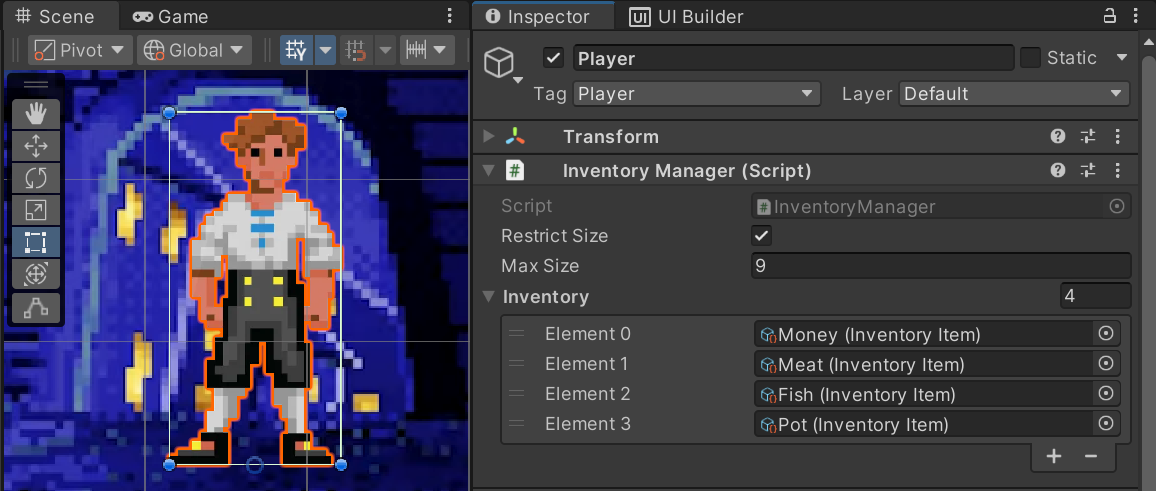
\includegraphics[width=1\linewidth]{img/User doc/inventory.png}
\caption{Inventory Manager inspector.}
\label{fig:Manual-Inventory}
\end{figure}

Another component that takes care of visualizing the inventory is \textbf{Display Inventory}. There is an option to set between two types of inventory: \textit{Name} or \textit{Icon}. The former displays the inventory items as a label with the word (or their combination), whereas the latter creates an icon depicting the item. Both of these approaches are used in the \textit{BaSS} and \textit{TSoMI} scenes.

Afterwards, the layout settings can be seen. These can adjust the configuration of the inventory slots: the starting location, width, height, and more. 

Finally, the \textit{Max Item Count} option sets how many items can be visible at most. It ties directly to the last script in the inventory system called \textbf{Inventory Scroll Button}, which when attached to a \verb|GameObject| lets us define the behavior of scrolling through the inventory by pressing an arrow. This exact scenario is used in \textit{TSoMI} scene.

\subsection{Dialogue System}
\label{Manual:DS}
The dialogue system provides the necessary tools for creating and managing conversations between characters. Dialogues are represented as dialogue graphs, which can be created in the \verb|Assets| folder by right-clicking and selecting \verb|Create > Dialogue > Dialogue Graph|. Once opened, the asset displays a dedicated editor window, as shown in Figure \ref{fig:Manual-DW}.

\begin{figure}[H]
\centering
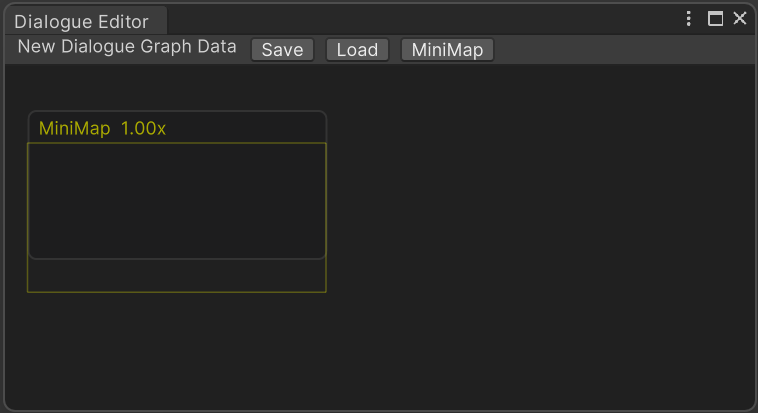
\includegraphics[width=0.8\linewidth]{img/User doc/image_2025-07-04_123651622.png}
\caption{Dialogue graph window.}
\label{fig:Manual-DW}
\end{figure}

At the top of the window is a panel that displays the file name along with three buttons. The first, \textit{Save}, stores the current state of the graph. If the window is closed without pressing this button, any unsaved changes will be lost. The second button, \textit{Load}, reloads the last saved version of the graph. This means that any edits made since the last save will be discarded. The third button, \textit{MiniMap}, toggles the visibility of a small map in the top-left corner of the editor window, which provides an overview of the graph layout.

\subsubsection{Nodes}
To add elements to the dialogue graph, press the Space key, which opens a search window. This interface allows the creation of either a \textit{Node} or a \textit{Group}. Selecting the \textit{Node} option presents six different node types to choose from. All node types support naming and include the option to generate a corresponding boolean variable called \textit{Visited}. This variable tracks whether the node has been accessed during a conversation, enabling conditional behavior based on the history of dialogues.

A new \textit{Visited} variable can be created by clicking the \textit{+} button next to its field in the node's configuration. The asset is automatically stored at the following path: \verb|Assets/Variables/Visited/[GraphName]|, where \verb|[GraphName]| corresponds to the name of the dialogue graph. The filename of the \textit{Visited} variable is either the node’s custom ID (if specified) or its unique GUID. For this reason, it is recommended to assign an ID to the node before creating the \textit{Visited} variable. Otherwise, the nodes have a very different structure from one another. In the rest of this Section, each type of node will be closely examined with Figures \ref{fig:Manual-Nodes1} and \ref{fig:Manual-Nodes2} providing visual guidance.

\begin{itemize}
    \item The \textbf{Start node }is a straightforward element in the dialogue graph. Aside from allowing the assignment of an ID and a corresponding \textit{Visited} variable, it features a single output port. Only one Start node is required per graph, any additional Start nodes will be ignored. This node functions only as an entry point, indicating where the dialogue begins inside the graph.
    \item In addition to the basic functionality common to all nodes, the \textbf{Event node} includes an \textit{Add Event} button. As the name implies, clicking this button adds a new slot for an associated \textbf{EventScriptableObject}, which references a \verb|ScriptableObject| used to trigger events. Since dialogue graphs are assets and cannot directly reference scene objects, this mechanism establishes the necessary link between the dialogue system and the game scene. A dialogue event \verb|ScriptableObject| can be created via the menu path: \verb|Create > Dialogue > Dialogue Event|. To bind this \verb|ScriptableObject| to the scene, a \verb|GameObject| in the scene must include the \textbf{Event Listener} component. This component maintains a list of pairs, where each pair consists of an event \verb|ScriptableObject| and a corresponding Unity Event that is invoked when the event is triggered. 
    \item The \textbf{Branch node} enables conditional branching, which allows the conversation flow to change based on the defined criteria. A new condition can be added by clicking the \textit{Add Condition} button and selecting one of four available types: boolean, integer, float, or string. Afterwards, a new field appears at the bottom of the node, which allows us to specify the expected value for that condition. The node includes two output ports labeled \textit{True} and \textit{False}. If all defined conditions are satisfied, the graph continues along the \textit{True} output. If any condition fails, the flow proceeds through the \textit{False} output instead. 
    \item The \textbf{Dialogue node} provides the actual lines of dialogue spoken by characters. Initially, the node contains a single input and output port, as well as a setting labeled \textit{Continue Style}. You can choose between two options: \textit{Wait} or \textit{Button}. The \textit{Wait} option allows you to specify a duration (in seconds) for which the dialogue remains on screen before automatically continuing. The \textit{Button} option, on the other hand, enables us to define a button that, when clicked, progresses the dialogue.

Additional dialogue entries can be added using the \textit{Add Text} button. Each entry consists of a pair: a \textit{Character ID} and a \textit{Dialogue Text} field. The \textit{Character ID} takes a reference to a \verb|ScriptableObject| of type \textbf{CharacterID}, which can be created by right-clicking in the \verb|Assets| folder and selecting \verb|Create > Dialogue > Character ID|. This object allows setting up the character's name, text offset, and text text color—settings that control how the text is displayed on screen. The actual binding of the ID to a specific \verb|GameObject| in the scene is explained later in this section. The \textit{Dialogue Text} field contains the line spoken by the character associated with the selected ID.

The Dialogue node also supports branching through dialogue choices. By clicking the \textit{Add Choice} button, additional output ports are generated. These are used exclusively to connect to \textit{Choice} nodes, which enable the player to select from multiple dialogue options during gameplay.

    \item The \textbf{Choice node} connects exclusively to additional output ports of a Dialogue node and is used to present clickable options to the player during dialogue sequences. It contains a text field where we specify the content of the choice that will be shown on screen. Similar to the Branch node, the Choice node allows the addition of conditions that determine whether the choice is visible or interactable during gameplay. 
    \item  The final node type is the \textbf{End node}, which is responsible for terminating the dialogue flow. It offers three options: ending the conversation entirely, repeating the last Dialogue node, or returning to the Start node. Regardless of the selected behavior, the End node does not contain any output ports, since it marks the end of a given dialogue path. 
\end{itemize}
\begin{figure}[H]
\centering
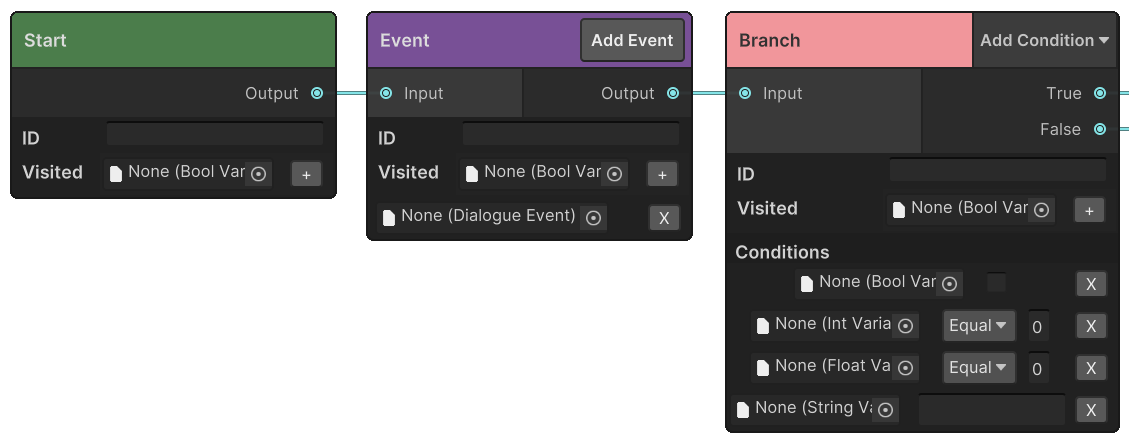
\includegraphics[width=1\linewidth]{img/User doc/nodes1.png}
\caption{Start, Event and Branch nodes.}
\label{fig:Manual-Nodes1}
\end{figure}
\begin{figure}[H]
\centering
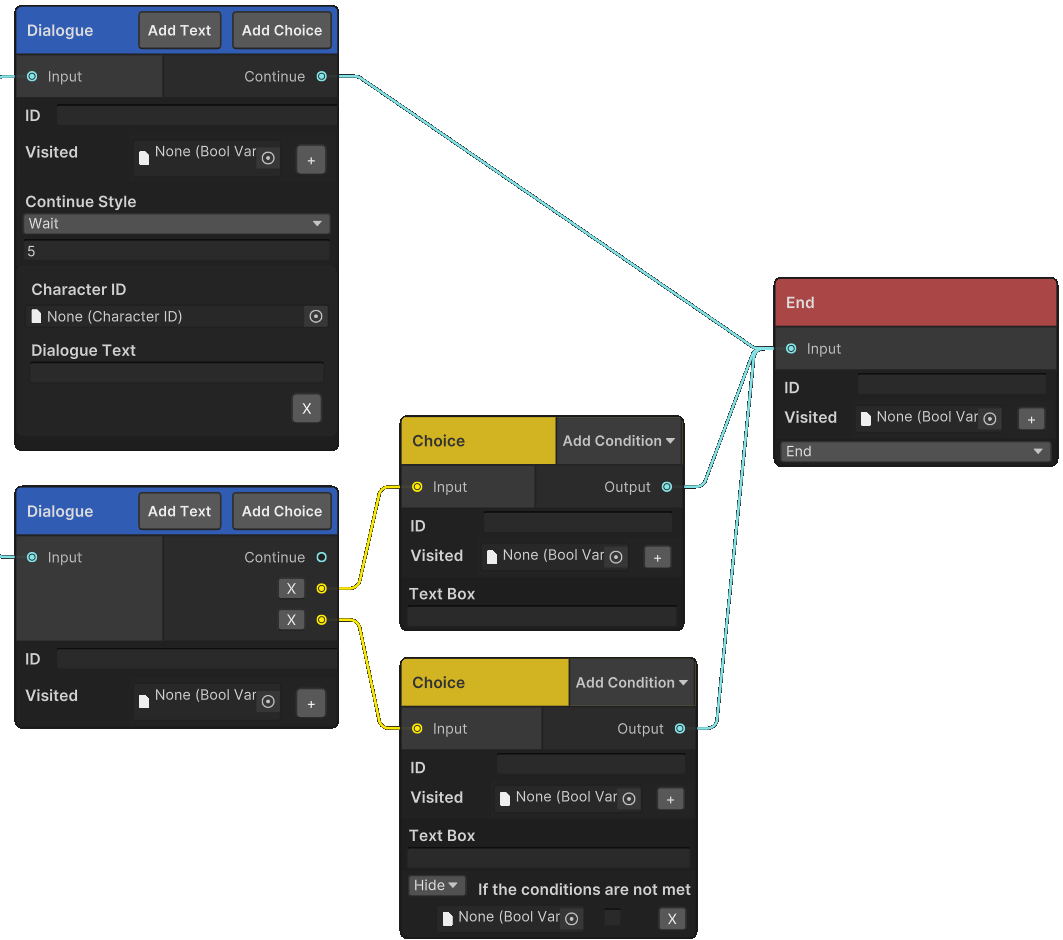
\includegraphics[width=1\linewidth]{img/User doc/nodes2.png}
\caption{Dialogue, Choice and End nodes.}
\label{fig:Manual-Nodes2}
\end{figure}

Both the \textit{TSoMI} and \textit{BaSS} scenes use the dialogue system, and it is recommended to take a look the dialogue graphs created for these showcase scenes, as they provide practical examples of how the system can be used. 

\subsubsection{Groups}
If you choose to create a new group from the search window via the path \verb|Groups > Base group|, a new box titled \textit{Dialogue Group} will appear in the editor. Nodes can be added to the group by clicking and holding the left mouse button on a node, dragging it into the group area, and then releasing the button. Multiple nodes can be added to a single group, and it is possible to create connections between any nodes, even those outside the group. When a node is part of a group, moving the group box will also move the contained nodes. To remove a node from the group, the node needs to be dragged outside of the group while holding the Shift key. A group can be renamed by double-clicking on its title. 

\subsubsection{Dialogue Control}
In order to run a conversation, the scene must contain a \verb|GameObject| with the \textbf{Dialogue Controller} component attached. This component is responsible for initiating the dialogue and also triggers Unity Events defined in its Inspector both at the beginning and at the end of the conversation. 

Using a Dialogue node in a dialogue graph, you can associate a line of text with a specific character through a \textbf{CharacterID} asset. To establish the link between a \verb|GameObject| in the scene and ensure that the dialogue text is displayed near the correct character, the \textbf{Dialogue Controller} component provides a list called \textit{Character ID Data}. Each entry in this list maps a \verb|GameObject| (referred to as the \textit{Character}) to a corresponding \textbf{CharacterID} asset (referred to as the \textit{ID}).

The \textbf{Dialogue UI Controller} component allows you to assign a specific prefab to be instantiated as the dialogue text box during runtime. Additionally, it provides options in the Inspector for customizing UI elements, such as button colors and other minor UI settings.
